% ============================================================
%  BAB 4 – HASIL PENELITIAN DAN PEMBAHASAN
%  Compile standalone:  pdflatex bab-4.tex
%  Compile as part of thesis: pdflatex main.tex
% ============================================================
\documentclass[main]{subfiles}
\usepackage{hyphenat}
\usepackage{iftex}

% ── Encoding, Language & Fonts ───────────────────────────────
\ifXeTeX
    \usepackage{polyglossia}
    \setmainlanguage{bahasai}
    \usepackage{fontspec}
    \setmainfont{TeX Gyre Termes}
    \setsansfont{TeX Gyre Heros}
    \setmonofont[Scale=0.88]{TeX Gyre Cursor}
\else
    \usepackage[utf8]{inputenc}
    \usepackage[T1]{fontenc}
    \usepackage[indonesian]{babel}
    \usepackage{mathptmx}
    \usepackage{helvet}
    \usepackage{courier}
\fi

% ── Page geometry (A4, UI thesis margins) ────────────────────
\usepackage[
  a4paper,
  top    = 2.54cm,
  bottom = 2.54cm,
  left   = 3.17cm,
  right  = 2.54cm
]{geometry}

% ── Line spacing & paragraph ─────────────────────────────────
\usepackage{setspace}
\onehalfspacing
\setlength{\parindent}{1.27cm}
\setlength{\parskip}{0pt}

% ── Microtype & justification ────────────────────────────────
\usepackage{microtype}
\sloppy

% ── Headings ─────────────────────────────────────────────────
\usepackage{titlesec}

\titleformat{\chapter}[block]
  {\centering\sffamily\bfseries\large}{}
  {0pt}{\MakeUppercase}
\titlespacing*{\chapter}{0pt}{0pt}{1.5em}

\titleformat{\section}
  {\sffamily\bfseries\normalsize}{\thesection}{1em}{}
\titlespacing*{\section}{0pt}{1.2em}{0.6em}

\titleformat{\subsection}
  {\sffamily\bfseries\normalsize}{\thesubsection}{1em}{}
\titlespacing*{\subsection}{0pt}{1em}{0.5em}

\titleformat{\subsubsection}
  {\sffamily\bfseries\normalsize}{\thesubsubsection}{1em}{}
\titlespacing*{\subsubsection}{0pt}{0.8em}{0.4em}

% ── Tables ───────────────────────────────────────────────────
\usepackage{longtable, booktabs, array, multirow}
\usepackage{calc}
\usepackage{tabularx}

% ── Math ─────────────────────────────────────────────────────
\usepackage{amsmath, amssymb}

% ── Graphics ─────────────────────────────────────────────────
\usepackage{graphicx}
\makeatletter
\def\maxwidth{\ifdim\Gin@nat@width>\linewidth\linewidth\else\Gin@nat@width\fi}
\makeatother
\setkeys{Gin}{width=\maxwidth,keepaspectratio}

% ── Lists ────────────────────────────────────────────────────
\usepackage{enumitem}
\setlist[enumerate,1]{
  label      = \arabic*.,
  leftmargin = 1.27cm,
  itemsep    = 4pt,
  parsep     = 0pt,
  topsep     = 4pt
}
\setlist[enumerate,2]{
  label      = \alph*.,
  leftmargin = 1.27cm,
  itemsep    = 3pt,
  parsep     = 0pt,
  topsep     = 2pt
}

% ── Hyperlinks ───────────────────────────────────────────────
\usepackage[hidelinks]{hyperref}

% Bibliography setup is inherited from main.tex (biblatex + references.bib)
% when this file is compiled standalone via the subfiles class.

% ============================================================
\begin{document}

% When standalone: set counter so \chapter{} renders as "BAB 4".
% When in main.tex: main.tex sets the counter before \subfile{bab-4}.
\ifSubfilesClassLoaded{}{\setcounter{chapter}{3}}

\chapter{Hasil Penelitian dan Pembahasan}

Bab ini memaparkan hasil penerapan kerangka kerja \textit{Knowledge Graph
Completion} berbasis \textit{Large Language Model} yang telah dirancang pada bab
sebelumnya, mulai dari pembangunan \textit{knowledge graph} melalui \textit{pipeline}
ekstraksi, konstruksi, dan \textit{completion}, hingga evaluasi kualitasnya.
Mengikuti kerangka \textit{Design Science Research} (DSR), pembahasan disusun
dengan menyajikan hasil tiap tahapan \textit{pipeline} beserta artefak yang
dihasilkannya (Subbab~\ref{sec:ingestion}--\ref{sec:instrumen-evaluasi}), yang kemudian dilanjutkan dengan evaluasi
struktural graf, validasi pakar, dan pembahasan kualitatif atas kualitas
relasi lintas-buku yang ditemukan (Subbab~\ref{sec:hasil-evaluasi}).

% ============================================================
\section{Tahap Ingestion (PDF Parsing)}\label{sec:ingestion}
% ============================================================

Tahap ini mengubah \textit{e-book} PDF menjadi struktur data yang siap
diproses oleh LLM. Keluaran utama berupa teks per bab, metadata halaman,
daftar subbab, glosarium, dan materi pokok.

\begin{enumerate}
  \item \textbf{Ekstraksi teks PDF.} PDF dimuat menggunakan
        \texttt{SimpleDirectoryReader} (LlamaIndex) dengan \textit{backend}
        PyMuPDF, sehingga setiap halaman menjadi satu objek \texttt{Document}
        yang menyimpan \texttt{page\_label}.

  \item \textbf{Deteksi halaman TOC (daftar isi).} Halaman diklasifikasikan
        sebagai TOC menggunakan heuristik dua-sinyal yang mencegah
        \textit{false positive} pada halaman konten biasa; detail
        implementasi disajikan di Lampiran A.

  \item \textbf{Parsing struktur Bab dan Subbab.} Pola Bab diekstrak dengan
        \textit{regex} yang menangkap format judul--\textit{leader dots}--nomor
        halaman (Contoh: ``Bab 4 Inovasi Bioteknologi..... 191''), sedangkan
        subbab diidentifikasi sebagai entri bertanda huruf besar (A., B., dst.)
        pada rentang TOC antara dua Bab berurutan. Hasil \textit{parsing}
        disusun sebagai daftar bab yang masing-masing memuat nama, halaman
        awal, dan daftar subbab.

  \item \textbf{Klasifikasi halaman TOC vs.\ konten.} Halaman yang terindikasi
        TOC pada deteksi awal digunakan untuk menyusun teks TOC gabungan,
        sementara halaman konten tidak disertakan agar \textit{parsing} bab dan
        subbab tetap stabil.

  \item \textbf{Ekstraksi glosarium.} Glosarium dicari pada 30 halaman terakhir
        menggunakan penanda \textit{state} \texttt{in\_glossary} yang diaktifkan
        oleh token ``glosarium'' dan dimatikan oleh terminator seperti
        ``indeks'' atau ``daftar pustaka''. Pasangan istilah--definisi yang
        ditemukan diuraikan menjadi \textit{lookup table}, yang kemudian dipakai
        sebagai validasi terminologi pada Tahap~2.

  \item \textbf{Penugasan bab ke \textit{chunk}.} Setiap \textit{chunk}
        dihubungkan ke bab berdasarkan interval halaman
        (\texttt{page\_start <= page < next\_page}), dengan \texttt{page\_label}
        dikonversi ke integer termasuk angka Romawi. Penugasan ini
        berkompleksitas $O(N \cdot C)$ untuk $N$ \textit{chunk} dan $C$ bab.

  \item \textbf{Ekstraksi materi pokok (Buku Guru).} Untuk tiap bab, sistem
        mencari \textit{region} teks yang sesuai judul bab di Buku Guru, lalu
        mengekstrak item di sekitar penanda ``Materi Pokok''. Hasilnya
        digunakan sebagai \textit{constraint} kurikulum pada Tahap~2 agar konsep
        yang diekstrak tetap sesuai kompetensi.
\end{enumerate}

% ============================================================
\section{Tahap Ekstraksi (LLM Prompting \& Schema)}\label{sec:ekstraksi}
% ============================================================

Tahap ini mengubah teks yang dihasilkan Tahap 1 menjadi \textit{knowledge
graph} terstruktur melalui \textit{schema-constrained prompting}.
Fokusnya adalah konsistensi struktur, validasi terminologi, dan
pembatasan konsep pada materi pokok.

\begin{enumerate}
  \item \textbf{Pemotongan teks (\textit{chunking}).}

  Teks dipecah menggunakan SentenceSplitter (LlamaIndex) dengan parameter
  sesuai Subbab~\ref{subsec:parameter-sistem}.

  \item \textbf{Agregasi per-bab.}

  \textit{Chunk} yang dipetakan ke bab yang sama digabungkan menjadi satu teks
  bab utuh, sehingga LLM memperoleh konteks bab secara penuh alih-alih potongan
  parsial per \textit{chunk}.

  \item \textbf{Ekstraksi triple.}

  Model: Gemini 2.5 Flash Lite via Google GenAI SDK. \textit{Prompt} bersifat
  \textit{few-shot} dan \textit{schema-constrained}. \textit{Prompt} menyertakan nama bab 
  beserta bab sebelum dan sesudahnya, daftar subbab dari daftar isi, glosarium sebagai 
  \textit{validation set}, materi pokok sebagai \textit{curriculum constraint}, konsep dari 
  buku lain sebagai \textit{cross-book context}, serta beberapa contoh \textit{triple} sebagai
  demonstrasi (\textit{few-shot}).

  \item \textbf{Struktur \textit{prompt}.}

  \textit{Prompt} didefinisikan \textit{inline} di dalam \textit{notebook} dan dibagi menjadi delapan blok:
  instruksi bahasa (keluaran wajib berbahasa Indonesia, kecuali istilah ilmiah
  tanpa padanan resmi); deklarasi hierarki graf (Kelas $\to$ Bab $\to$ Subbab
  $\to$ Konsep); filter konten (abaikan daftar isi, soal latihan, glosarium,
  rangkuman, dan elemen administratif); serta aturan ekstraksi konsep (delapan
  aturan), termasuk batas 3--5 konsep per subbab, deskripsi 1--2 kalimat ilmiah,
  dan validasi materi pokok Buku Guru.

  \item \textbf{Vokabulari relasi.}

  \textit{Prompt} membatasi ekstraksi relasi antar-konsep pada 15 tipe relasi
  intra-buku sesuai \textit{controlled vocabulary} ontologi
  (Subbab~\ref{subsec:skema-ontologi}); instruksi \textit{cross-chapter
  reasoning} secara terpisah menghasilkan relasi pedagogis antar-bab
  (PRASYARAT atau MEMPERSIAPKAN).

  \item \textbf{Penguraian keluaran terstruktur.}

  Respons LLM dibersihkan dari penanda \textit{markdown} lalu diuraikan dari
  format JSON menjadi objek terstruktur yang memuat ringkasan bab serta daftar
  konsep per subbab---lengkap dengan deskripsi, status validasi glosarium,
  rujukan materi pokok, tautan lintas-buku, dan relasi antar-konsep.

  \item \textbf{Validasi pascaproses.} Sebelum dikonstruksi ke graf, keluaran
  LLM melewati tiga penyaringan. \emph{Pertama}, penyaringan tautan lintas-buku:
  tautan ditolak apabila buku target sama dengan buku sumber atau buku target
  tidak termuat dalam korpus, sehingga mencegah \textit{self-loop} dan referensi
  \textit{dangling}. \emph{Kedua}, \textit{fallback} heuristik
  (\texttt{infer\_cross\_links}): bila LLM mengembalikan keluaran kosong, sistem
  menjalankan pencocokan tumpang-tindih token bergaya Jaccard, memakai token
  sepanjang minimal empat karakter dan non-\textit{stopword}, lalu mengambil dua
  pasangan konsep antarbuku dengan tumpang-tindih tertinggi. \emph{Ketiga},
  sanitasi relasi: \textit{triple} dengan tipe atau target kosong dibuang.
\end{enumerate}

% ============================================================
\section{Graph Construction (Eksekusi Neo4j Cypher)}\label{sec:graph-construction}
% ============================================================

Tahap ini membuat \textit{knowledge graph} ke Neo4j dengan strategi
tiga-\textit{pass} agar konsisten secara referensial dan idempoten.

\begin{enumerate}
  \item \textbf{Pass 1 --- Instansiasi node.}
  \begin{itemize}
    \item Node \texttt{Grade}, \texttt{Chapter}, \texttt{Subtopic}, dan
      \texttt{Concept} dibuat melalui operasi \texttt{MERGE}
      (\textit{idempotent upsert}).
    \item Properti node ditetapkan melalui klausa \texttt{ON CREATE} dan
      \texttt{ON MATCH}.
    \item Kunci \texttt{MERGE} gabungan (\texttt{name}, \texttt{grade}) menegakkan
      sifat \textit{shared node} pada \texttt{Concept} sebagaimana didefinisikan
      pada Subbab~\ref{subsec:skema-ontologi}.
  \end{itemize}

  \item \textbf{Tulang punggung hierarki.} Relasi struktural
  \texttt{HAS\_CHAPTER}, \texttt{HAS\_SUBTOPIC}, \texttt{HAS\_CONCEPT}, dan
  \texttt{NEXT\_CHAPTER} ditarik dari struktur daftar isi (bukan dari LLM)
  untuk menjamin keterurutan hierarki bab.

  \item \textbf{Pass 2 --- Relasi dalam-buku.}
  \begin{itemize}
    \item Relasi semantik antar-\texttt{Concept} ditanam dengan strategi
      dua-tingkat: apabila konsep target sudah berada dalam himpunan
      \texttt{Concept} buku yang sedang diproses, sistem membuat \textit{edge}
      langsung antar-\texttt{Concept}; jika belum, target direpresentasikan
      sebagai node \texttt{ConceptTarget} yang berperan sebagai
      \textit{placeholder}.
    \item Pemisahan label \texttt{Concept} dan \texttt{ConceptTarget}
      (Subbab~\ref{subsec:skema-ontologi}) memudahkan audit terhadap konsep yang
      belum ter-\textit{anchor} pada sumber tekstual.
    \item Tipe relasi dinormalisasi (karakter non-alfanumerik diganti garis
      bawah) agar sesuai dengan sintaksis \textit{relationship type} Cypher.
  \end{itemize}

  \item \textbf{Pass 3 --- Relasi lintas-buku.}
  \begin{itemize}
    \item \textit{Edge} lintas-buku diberi prefiks \texttt{LINTAS\_BUKU\_}
      diikuti tipe relasinya (mis.\ \texttt{LINTAS\_BUKU\_APLIKASI\_DARI}).
    \item Penjagaan integritas diterapkan: buku target harus berbeda dari buku
      sumber dan termuat dalam korpus yang diproses.
    \item Apabila konsep target belum ada pada \textit{scope} mata pelajaran
      tujuan, node \texttt{Concept} baru dibuat secara \textit{lazy}
      (\textit{lazy materialization}).
  \end{itemize}

  \item \textbf{Sifat idempoten.} Seluruh \textit{pass} menggunakan
  \texttt{MERGE} sehingga eksekusi ulang \textit{notebook} tidak menggandakan
  node maupun \textit{edge}. Properti ini penting agar eksperimen dapat
  dijalankan secara iteratif tanpa mengotori graf yang telah terbentuk.
\end{enumerate}

% ============================================================
\section{Graph Completion (Vector Index ANN \& LLM Classifier)}\label{sec:graph-completion}
% ============================================================

Tahap ini menemukan relasi implisit lintas-disiplin yang tidak ditangkap LLM
pada Tahap 2, mengikuti paradigma \textit{embedding} + \textit{retrieval} + \textit{LLM-as-classifier}.
Prosesnya terdiri dari empat sub-tahap: (1) \textit{concept embedding},
(2) \textit{candidate retrieval} via ANN, (3) \textit{candidate pruning},
dan (4) \textit{relation classification} via LLM.

\begin{enumerate}
  \item \textbf{Concept embedding.}

  Atribut \texttt{description} pada tiap \texttt{Concept} di-\textit{encode}
  menjadi vektor padat (\textit{dense vector}):
  \[
    \mathbf{e}_c \in \mathbb{R}^{d}, \quad d = 3072
  \]
  menggunakan model \textit{embedding} \texttt{gemini-embedding-001} melalui Google GenAI SDK.
  Representasi vektor ini memetakan semantik teks ke ruang Euclidean berdimensi
  tinggi sehingga konsep yang secara makna berkaitan akan memiliki vektor yang
  berdekatan. Vektor yang dihasilkan disimpan sebagai properti node (embedding) di
  Neo4j dan diindeks menggunakan Neo4j Vector Index. Perlu ditegaskan bahwa
  \textit{embedding} ini bersifat semantik (diturunkan dari deskripsi tekstual
  konsep) sehingga berbeda dari \textit{embedding} struktural berbasis topologi
  graf yang keterbatasannya dibahas pada Subbab~\ref{subsec:kgc}. Selain itu,
  \textit{embedding} di sini hanya berperan sebagai penyaring kandidat, sedangkan
  keputusan akhir relasi tetap ditentukan oleh LLM.

  Pengindeksan memanfaatkan algoritma HNSW (lihat Subbab~\ref{subsec:kgc}), yang
  struktur graf berlapisnya diilustrasikan pada Gambar~\ref{fig:hnsw}. Parameter
  HNSW tidak dikonfigurasi secara eksplisit pada \texttt{CREATE VECTOR INDEX},
  sehingga Neo4j menerapkan nilai \textit{default} ($M = 16$,
  \texttt{ef\_construction} $= 100$) dengan \textit{vector quantization} aktif
  untuk mengoptimalkan penggunaan memori.

  \begin{figure}[htbp]
    \centering
    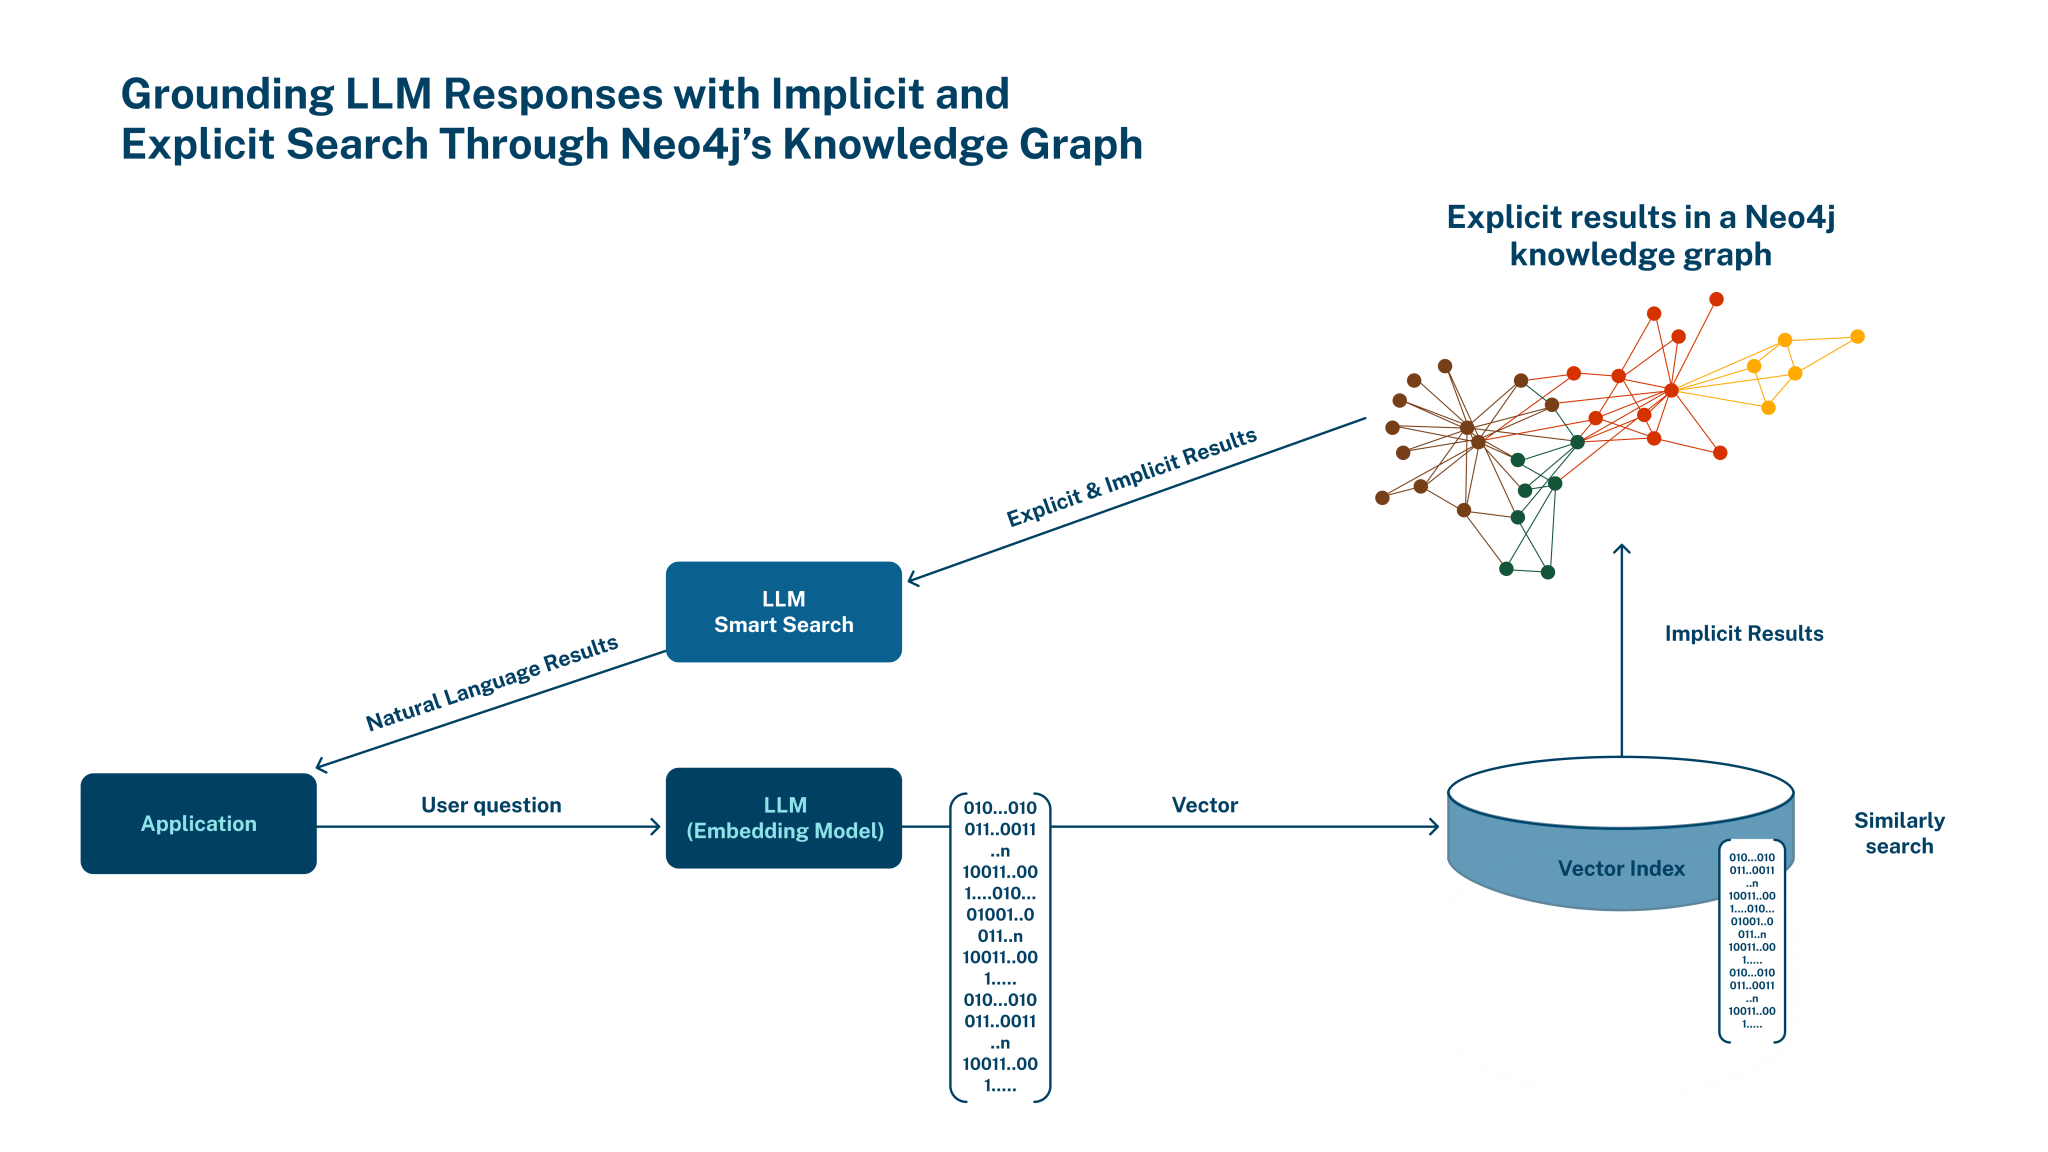
\includegraphics[width=\maxwidth]{images/media/image23.png}
    \caption{Ilustrasi struktur graf berlapis HNSW pada Neo4j Vector Index 
    (diadaptasi dari \textcite{malkov_efficient_2020}).}
    \label{fig:hnsw}
  \end{figure}

  \item \textbf{Candidate retrieval via ANN (Approximate Nearest Neighbor).}

  Untuk tiap \textit{query} node $q$, dijalankan pencarian ANN pada Neo4j Vector Index
  yang mengembalikan top-$k$ node terdekat berdasarkan \textit{cosine similarity}
  (didefinisikan pada Subbab~\ref{subsec:kgc}). Sebaran nilai \textit{cosine
  similarity} antar pasangan konsep pada indeks ditunjukkan pada
  Gambar~\ref{fig:cosine-scatter}.

  \begin{figure}[htbp]
    \centering
    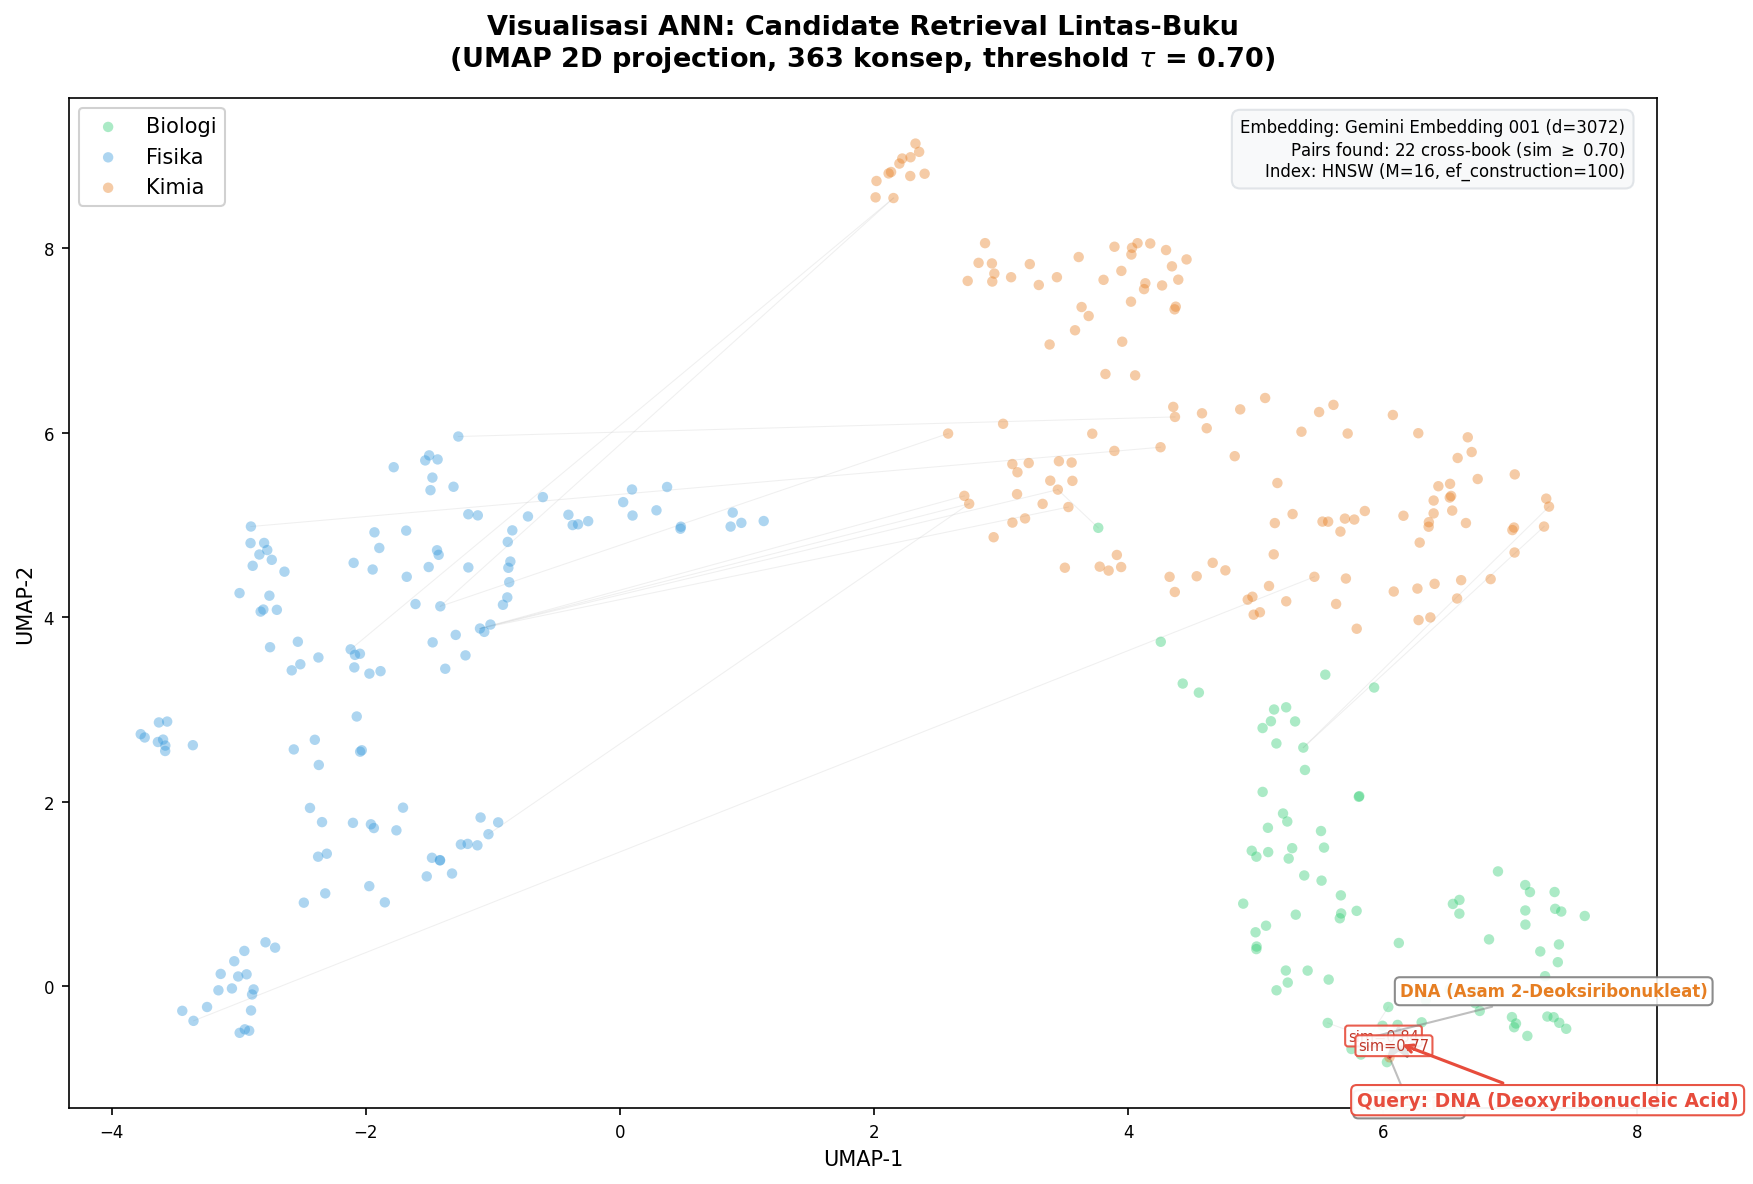
\includegraphics[width=\maxwidth]{images/media/image5.png}
    \caption{Sebaran \textit{cosine similarity} antar pasangan konsep pada indeks vektor.}
    \label{fig:cosine-scatter}
  \end{figure}

  Hanya pasangan dengan $\text{sim} \geq \tau$ (dengan $\tau = 0{,}70$ untuk
  pencarian lintas-buku) yang lolos ke tahap berikutnya:
  \[
    \text{candidates}(q)
    = \bigl\{\, c \in \mathcal{C} \;\big|\; \text{sim}(\mathbf{e}_q,\, \mathbf{e}_c) \geq \tau \,\bigr\}
  \]
  Berkat indeks HNSW (Subbab~\ref{subsec:kgc}), pencarian kandidat menghindari
  perbandingan \textit{pairwise} $O(n^2)$ sehingga tetap \textit{tractable} pada
  skala ratusan hingga ribuan konsep.

  \item \textbf{Candidate pruning.}

  Pasangan kandidat yang lolos ANN disaring melalui empat filter sebelum
  diklasifikasi LLM:
  \begin{enumerate}[label=\roman*.]
    \item \textit{Eksklusi self-pair}: kueri ANN mencegah sebuah node
      menjadi kandidat bagi dirinya sendiri.
    \item \textit{Deduplikasi}: setiap pasangan dinormalisasi menjadi urutan
      tetap sehingga $(A,B)$ dan $(B,A)$ diperlakukan identik dan hanya diproses
      sekali.
    \item \textit{Penyaringan lintas-mapel}: pasangan dari mata pelajaran yang
      sama dibuang karena relasi dalam-mapel telah ditangani pada Tahap~2,
      sehingga tahap \textit{completion} hanya mencari jembatan antardisiplin.
    \item \textit{Penyaringan relasi tertipe}: pasangan yang sudah memiliki
      \textit{edge} bertipe (selain \texttt{SIMILAR\_TO}) dibuang untuk mencegah
      duplikasi relasi.
  \end{enumerate}
  Tahap \textit{pruning} ini secara signifikan menekan jumlah pasangan yang
  diumpankan ke LLM, sehingga mengurangi biaya inferensi dan menjaga
  \textit{precision}.

  \item \textbf{Relation classification via LLM.}

  Tiap pasangan yang lolos \textit{pruning} diklasifikasikan oleh LLM
  (Gemini 2.5 Flash Lite) melalui \textit{prompt few-shot} yang memuat: (1)
  deskripsi dan konteks kedua konsep (nama, deskripsi, mata pelajaran); (2)
  konteks graf berupa bab asal, hingga lima \textit{edge} keluar yang sudah ada,
  serta tetangga bersama (\textit{shared neighbors}); dan (3) definisi ketat tiap
  label target. Untuk klasifikasi lintas-buku, LLM memilih salah satu dari lima
  label semantik \texttt{LINTAS\_BUKU\_*} yang didefinisikan pada
  Subbab~\ref{subsec:skema-ontologi}, atau label \texttt{none} apabila kemiripan
  semantik hanya superfisial sehingga tidak ada relasi kurikuler bermakna.
  Klasifikasi dilengkapi skor \textit{confidence} dalam rentang $[0, 1]$. Hasil
  klasifikasi di-\textit{cache} dengan kunci yang tidak bergantung pada urutan
  pasangan dan menyertakan \textit{sidik jari} (\textit{hash}) konteks graf,
  sehingga perubahan graf otomatis memicu klasifikasi ulang.


  \item \textbf{Edge writeback.}

  Hanya pasangan dengan label non-none yang dituliskan kembali sebagai \textit{edge}
  baru ke Neo4j beserta properti \textit{confidence score}, description (satu kalimat
  \textit{rationale} Bahasa Indonesia), dan method (identifier model dan versi
  \textit{prompt}). Strategi ini melengkapi graf tanpa menambah \textit{noise} terstruktur,
  menghasilkan \textit{knowledge graph} yang lebih lengkap secara topologis sambil
  menjaga kualitas relasi melalui \textit{gating} LLM.
\end{enumerate}

% ============================================================
\section{Arsitektur Instrumen Evaluasi}\label{sec:instrumen-evaluasi}
% ============================================================

Untuk mengukur efektivitas dan kualitas \textit{Knowledge Graph} (KG) yang telah
dibangun, penelitian ini mengembangkan instrumen evaluasi khusus yang
terdiri dari dua komponen arsitektur utama: kalkulasi metrik struktural
berbasis \textit{Cypher} dan aplikasi web KG Review App untuk validasi pakar.

\begin{enumerate}
  \item \textbf{Implementasi Kalkulasi Struktural pada Neo4j Aura.}

  Seluruh perhitungan metrik topologi graf dieksekusi secara langsung di sisi
  basis data menggunakan kueri \textit{Cypher} pada Neo4j Aura. Pendekatan
  eksekusi \textit{database-side} ini memastikan bahwa metrik dapat diturunkan ulang
  setiap saat melalui kueri \textit{read-only}. Pendekatan ini dirancang khusus agar
  kompatibel dengan spesifikasi tier Aura Free yang tidak menyertakan pustaka
  \textit{Graph Data Science} (GDS), sehingga hasil perhitungannya dapat langsung
  diintegrasikan ke dalam \textit{dashboard} visualisasi.

  \item \textbf{Arsitektur KG Review App (Next.js dan Redis).}

  Untuk memfasilitasi evaluasi intrinsik oleh pakar (\textit{human evaluation}),
  dikembangkan sebuah aplikasi web kustom bernama KG Review App. Dari sisi
  \textit{frontend}, aplikasi ini dibangun menggunakan kerangka kerja Next.js berbasis
  React yang mendukung \textit{server-side rendering}. Pada sisi \textit{backend}, \textit{route
  handler} Next.js dikonfigurasi untuk berkomunikasi secara asinkron dengan
  Redis yang bertindak sebagai \textit{primary key-value store}.

  Redis dipilih karena latensinya yang sangat rendah, menjadikannya ideal untuk
  menangani \textit{payload} berukuran kecil seperti \textit{rating} per-triple dan
  fitur \textit{auto-save}; setiap aksi penilaian pakar memicu \textit{debounced
  auto-save} otomatis sehingga sesi dapat dilanjutkan tanpa arsitektur relasional
  yang kompleks. Skema kunci dan diagram arsitektur lengkap disajikan di Lampiran B.

  \begin{figure}[htbp]
    \centering
    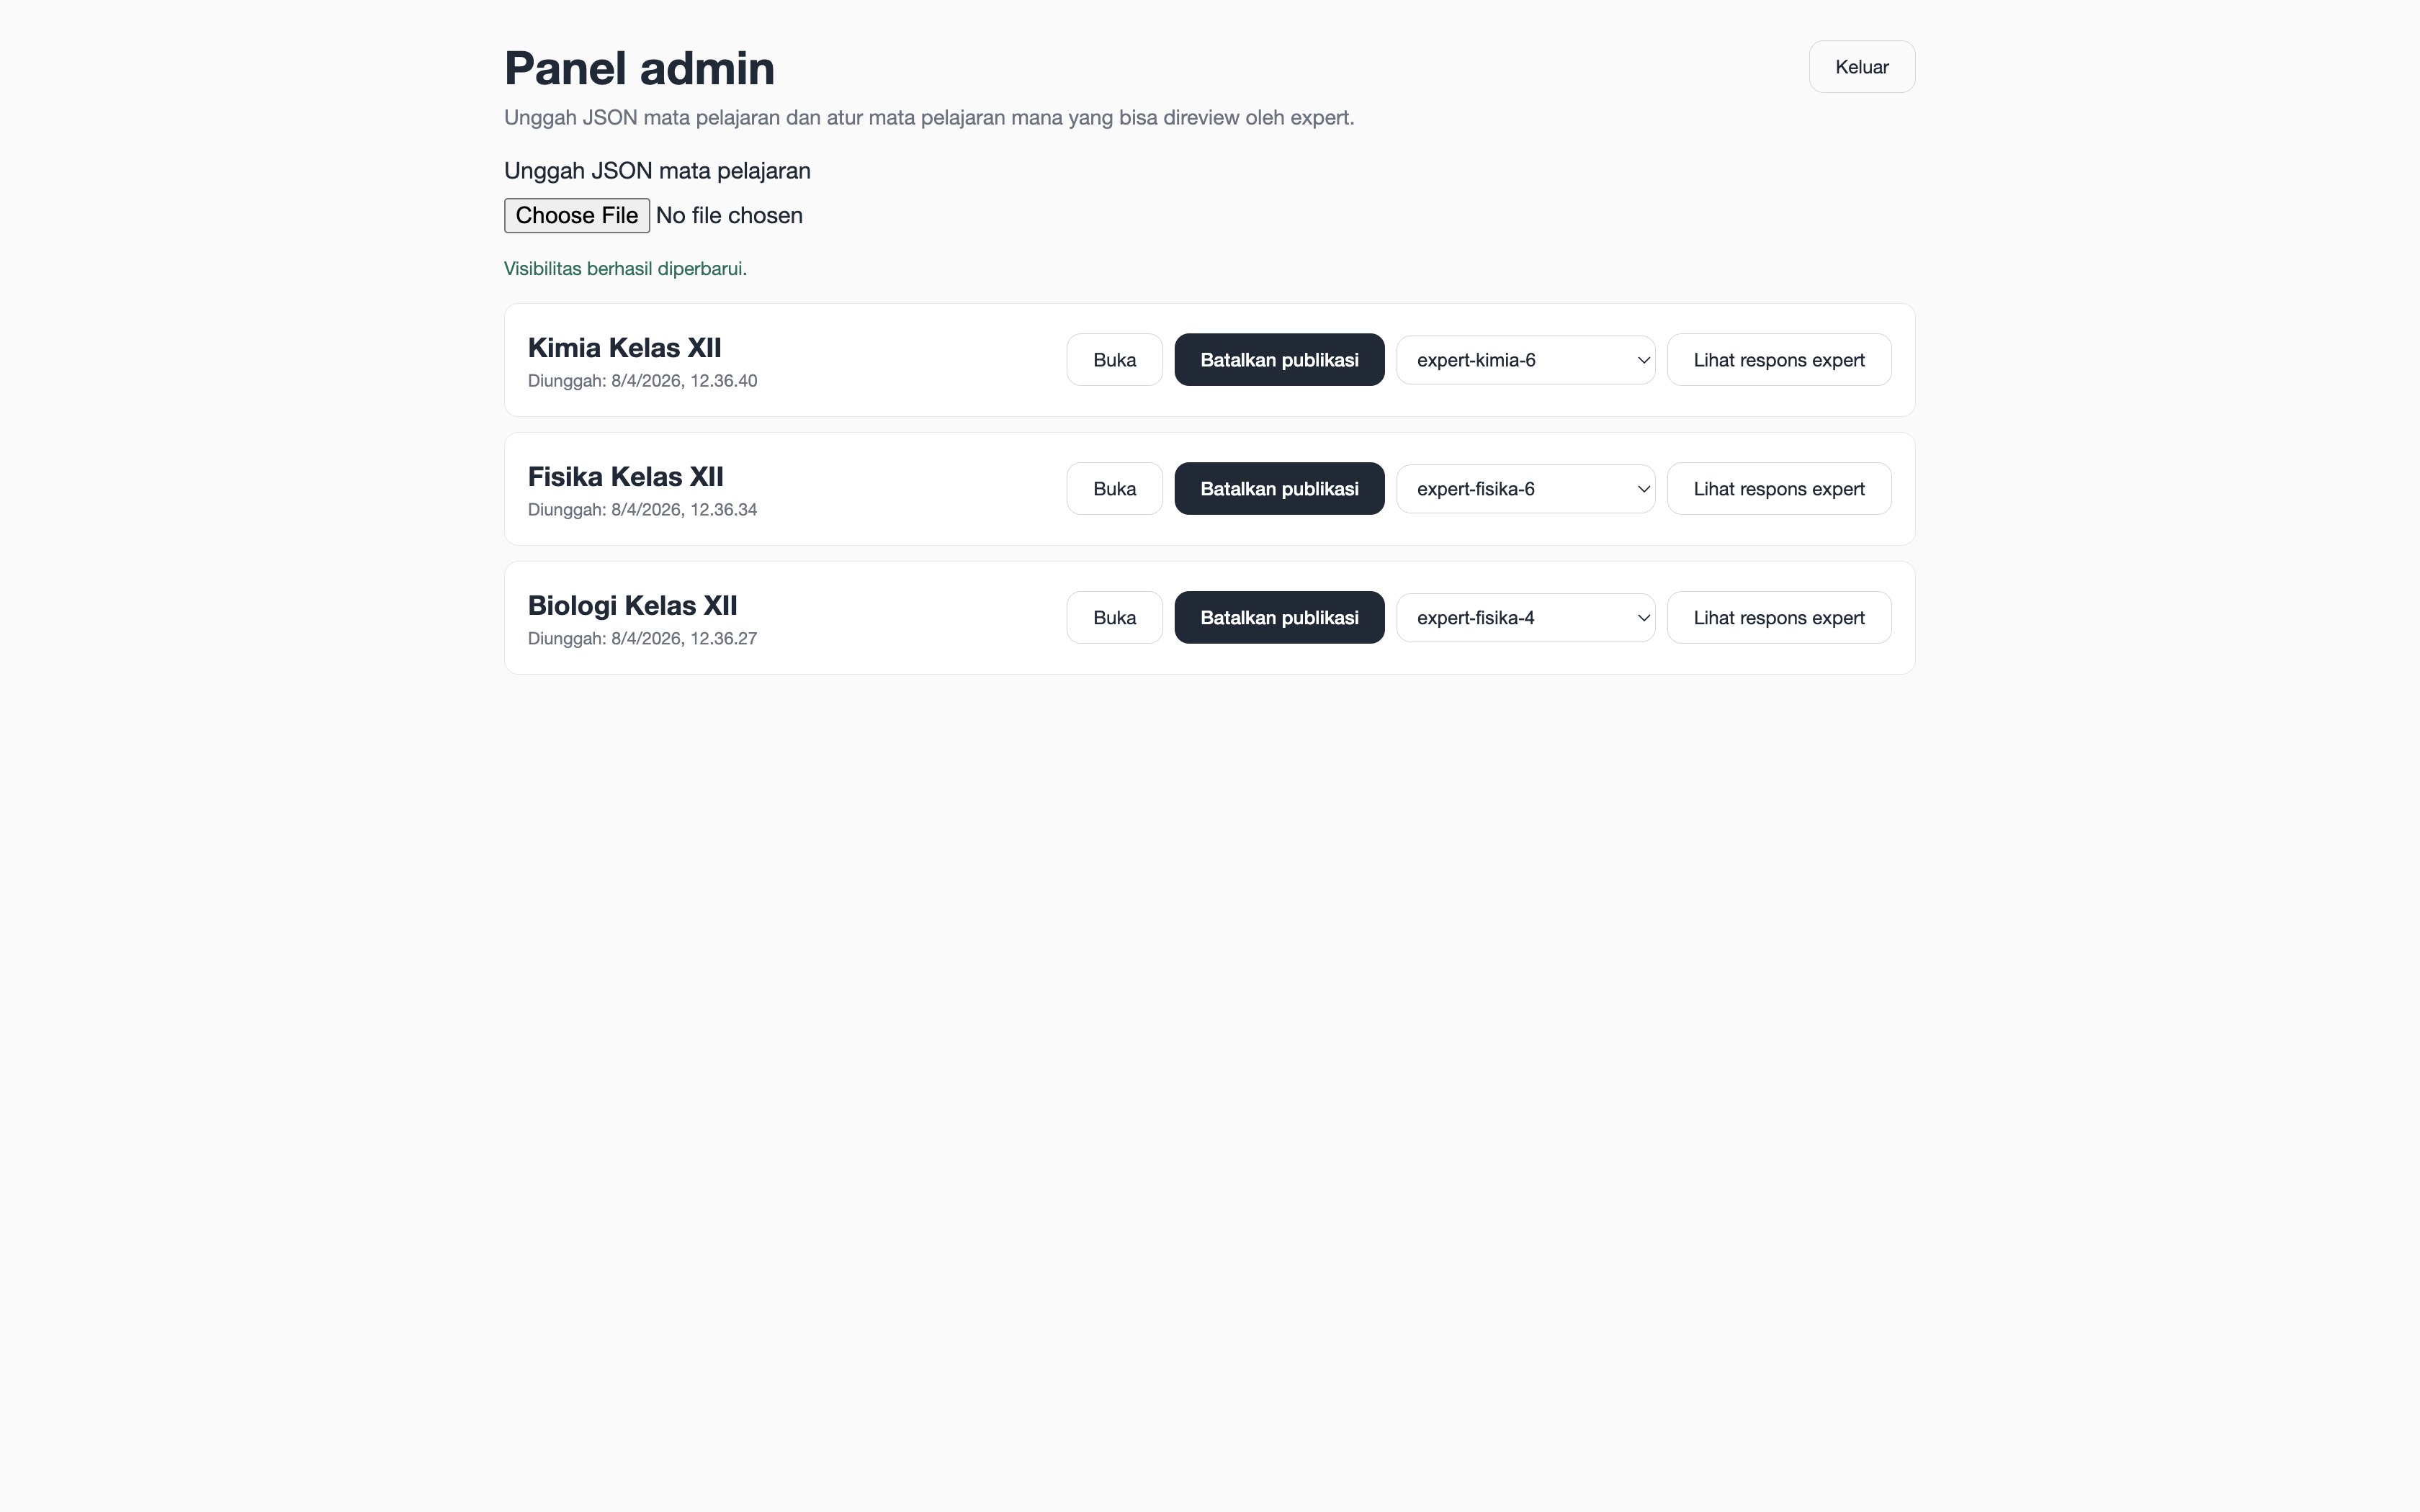
\includegraphics[width=\maxwidth]{images/media/image13.png}
    \caption{Tampilan dasbor Admin untuk mengunggah graf JSON pada KG Review App.}
    \label{fig:admin-dashboard}
  \end{figure}

  \item \textbf{Role-Based Access Control (RBAC).}

  Untuk menjaga integritas proses validasi, arsitektur aplikasi menerapkan
  kontrol akses berbasis peran (RBAC) dengan dua peran utama:
  \begin{enumerate}
    \item Admin: memiliki hak akses manajerial untuk mengunggah berkas JSON
      hasil ekstraksi (Tahap 3 dan 4) ke dalam sistem per mata pelajaran,
      mengatur status publikasi graf, serta melihat panel metrik (tinjauan
      respons) dari para pakar dalam mode \textit{read-only}.
    \item Expert (Reviewer): memiliki hak akses \textit{read-write} operasional untuk
      memberikan \textit{rating} pada setiap triple relasi yang disajikan, serta
      memberikan masukan jika ada triple esensial yang hilang (\textit{missing
      triples}) melalui form penambahan.
  \end{enumerate}

  \item \textbf{Desain Skema Validasi Dua Fase.}

  Mengingat kompleksitas ontologi kurikulum sains, antarmuka evaluasi untuk
  Expert dirancang menggunakan skema studi dua fase guna menurunkan beban
  kognitif (\textit{cognitive load}) penilai:
  \begin{enumerate}
    \item \textbf{Fase 1 (Validasi Intra-Mapel):} pakar mengevaluasi kualitas
      hierarki dan relasi semantik secara spesifik di dalam lingkup satu
      mata pelajaran (misalnya Fisika saja).
    \item \textbf{Fase 2 (Interkoneksi Antar-Mapel):} pakar secara khusus
      mengevaluasi validitas relasi implisit lintas-disiplin sains
      (berlabel \texttt{LINTAS\_BUKU\_*}) yang diprediksi oleh LLM pada tahap
      \textit{completion}. Pemisahan fase ini memungkinkan analisis data yang lebih
      terisolasi dan akurat.
  \end{enumerate}
\end{enumerate}

% ============================================================
\section{Hasil Evaluasi dan Pembahasan}\label{sec:hasil-evaluasi}
% ============================================================

Tahap evaluasi dalam kerangka \textit{Design Science Research} (DSR) ini
bertujuan untuk mengukur performa dan kualitas \textit{Knowledge Graph}
(KG) yang dihasilkan oleh \textit{pipeline} sistem. Evaluasi dilakukan secara
komprehensif melalui analisis kuantitatif terhadap topologi graf,
validasi kualitatif oleh pakar domain, pembahasan mendalam terkait
\textit{error} model LLM, serta komparasi antar-disiplin ilmu sains.

% ────────────────────────────────────────────────────────────
\subsection{Hasil Analisis Struktural Graf}\label{subsec:struktural}
% ────────────────────────────────────────────────────────────

\begin{figure}[htbp]
  \centering
  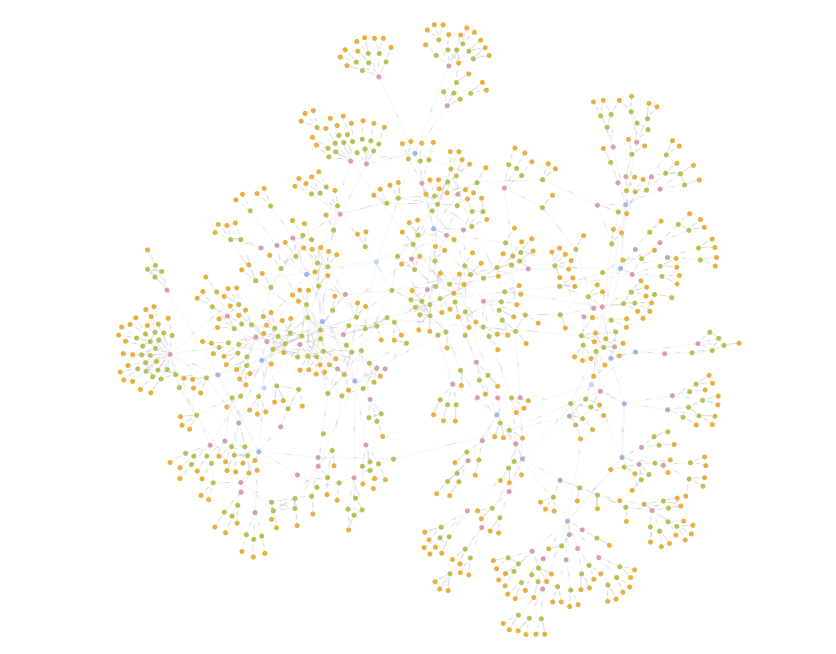
\includegraphics[width=\maxwidth]{images/media/image21.png}
  \caption{Visualisasi topologi keseluruhan \textit{knowledge graph} hasil konstruksi.}
  \label{fig:kg-topologi}
\end{figure}

Analisis struktural bertujuan untuk mengevaluasi kualitas interkoneksi
jaringan pengetahuan secara matematis, khususnya untuk melihat
perbandingan struktur graf sebelum \textit{Knowledge Graph Completion} (pre-KGC)
dan sesudahnya (post-KGC). Seluruh perhitungan pada bagian ini
dieksekusi melalui kueri \textit{Cypher} di Neo4j dengan berpedoman pada
formulasi metrik topologi yang telah dijelaskan pada Subbab~\ref{subsec:metrik-topologi}.

\begin{longtable}{@{}
  >{\raggedright\arraybackslash}p{0.38\linewidth}
  >{\centering\arraybackslash}p{0.27\linewidth}
  >{\centering\arraybackslash}p{0.27\linewidth}@{}}
\caption{Perbandingan metrik struktural pre-KGC dan post-KGC.}
\label{tab:struktural}\\
\toprule
\textbf{Metrik Struktural} & \textbf{Pre-KGC} & \textbf{Post-KGC} \\
\midrule
\endhead
ADC (seluruh node)                & 2{,}4123 & 2{,}6970 \\
ADC (Konsep-ke-Konsep)            & 0{,}7384 & 1{,}4651 \\
\textit{Graph Density}            & 0{,}00108 & 0{,}00214 \\
\textit{Modularity}               & 0{,}8106 & 0{,}3732 \\
\bottomrule
\end{longtable}

\begin{enumerate}
  \item \textbf{Evaluasi \textit{Average Degree Centrality} (ADC) dan Kepadatan.}

  Berdasarkan Tabel~\ref{tab:struktural}, ADC seluruh node meningkat dari 2{,}41
  (pre-KGC) menjadi 2{,}70 (post-KGC), suatu kenaikan sebesar 11{,}8\%. Namun
  peningkatan yang lebih signifikan terjadi pada ADC Konsep-ke-Konsep, yang hampir
  berlipat ganda dari 0{,}74 menjadi 1{,}47 (+98{,}7\%). Peningkatan ini
  mencerminkan bahwa \textit{pipeline} KGC berhasil menambahkan 125 relasi
  lintas-buku baru yang secara langsung menghubungkan node Concept antar-mapel,
  meningkatkan kepadatan interkoneksi semantik yang sebelumnya tidak ada.
  \textit{Graph Density} juga meningkat secara proporsional dari 0{,}00108 menjadi
  0{,}00214 (hampir dua kali lipat), konsisten dengan penambahan \textit{edge}
  lintas-buku tersebut. Nilai densitas yang masih sangat rendah pada kedua fase
  merupakan karakteristik umum \textit{knowledge graph} berukuran sedang-besar,
  karena hanya sebagian kecil dari seluruh kemungkinan pasangan konsep yang
  memiliki relasi bermakna \parencite{hogan_knowledge_2022}.

  \item \textbf{Evaluasi \textit{Modularity}.}

  Analisis struktur komunitas menggunakan metrik \textit{Modularity} pada fase
  pre-KGC mencatatkan nilai 0{,}811, yang mengindikasikan struktur komunitas yang
  sangat kuat --- ketiga komunitas mapel (Fisika, Kimia, Biologi) hampir sepenuhnya
  terisolasi satu sama lain, sejalan dengan kondisi \textit{siloed learning} yang
  diidentifikasi sebagai masalah penelitian. Setelah KGC, nilai \textit{Modularity}
  turun secara signifikan menjadi 0{,}373, menandakan bahwa relasi lintas-buku yang
  ditambahkan berhasil menjembatani ketiga komunitas tersebut dan mengurangi
  keterpisahan topologis antar-disiplin. Penurunan ini merupakan indikator
  keberhasilan utama \textit{pipeline}, karena penurunan \textit{Modularity}
  mencerminkan peningkatan interkoneksi lintas-komunitas sebagaimana dirumuskan
  pada Subbab~\ref{subsec:metrik-topologi}.

  \item \textbf{Evaluasi Metrik Ekstraksi dan Hubungan.}

  Di luar evaluasi topologi di atas, kualitas hasil ekstraksi LLM secara
  spesifik diukur menggunakan metrik \textit{Description Completeness} (DC),
  \textit{Empty SubKonsep Rate} (ESR), dan
  \textit{Typed Relation Ratio} (TRR) sebagaimana didefinisikan pada
  Subbab~\ref{subsec:metrik-ekstraksi} dan~\ref{subsec:metrik-hubungan}.
  Sistem mencatatkan nilai DC sebesar 93{,}07\% --- identik pada
  fase pre-KGC maupun post-KGC karena DC mengukur kualitas deskripsi node yang
  tidak berubah akibat penambahan \textit{edge} KGC. Metrik ESR tercatat 0\%
  (0,00) pada kedua fase --- jauh di bawah ambang maksimal 10\% --- yang
  menandakan bahwa seluruh entitas induk (\texttt{:Subtopic}) berhasil
  didekomposisi menjadi setidaknya satu konsep turunan, sehingga tidak ada
  ``node buntu'' dalam graf. Nilai TRR meningkat dari
  69{,}69\% (pre-KGC) menjadi 74{,}86\% (post-KGC), mencerminkan bahwa KGC
  menambahkan \textit{edge} bertipe semantik spesifik sehingga proporsi relasi
  bertype meningkat relatif terhadap total \textit{edge} dalam graf.
\end{enumerate}

% ────────────────────────────────────────────────────────────
\subsection{Hasil Validasi Pakar}\label{subsec:validasi-pakar}
% ────────────────────────────────────────────────────────────

Evaluasi performa sistem dalam mengekstrak dan memprediksi relasi
dievaluasi langsung oleh panel pakar (sebanyak 6 \textit{reviewer}) menggunakan
instrumen KG Review App. Berdasarkan desain studi dua fase, hasil
evaluasi dipisahkan menjadi evaluasi intra-mapel (Fase 1) dan inter-mapel
(Fase 2). Data dianalisis menggunakan metrik \textit{Precision}, \textit{Recall},
F1-Score, dan uji kesepakatan Gwet's AC1 yang merujuk pada Subbab~\ref{subsec:validasi-manusia}.

{\setlength{\tabcolsep}{4pt}
\begin{longtable}{@{}
  >{\raggedright\arraybackslash}p{0.16\linewidth}
  >{\raggedright\arraybackslash}p{0.13\linewidth}
  >{\centering\arraybackslash}p{0.11\linewidth}
  >{\centering\arraybackslash}p{0.09\linewidth}
  >{\centering\arraybackslash}p{0.09\linewidth}
  >{\centering\arraybackslash}p{0.09\linewidth}
  >{\centering\arraybackslash}p{0.09\linewidth}
  >{\centering\arraybackslash}p{0.09\linewidth}@{}}
\caption{Hasil validasi Fase 1 (intra-mapel) per penilai dan konsensus final.
  Kolom ``Final'' adalah konsensus setelah resolusi ketidaksepakatan via \textit{LLM-as-a-judge}.
  Jumlah ``Ditinjau'' pada baris Final lebih kecil daripada baris penilai karena
  \textit{triple} yang pada konsensus akhir dinilai gagal-ekstraksi/invalid
  (label ``Salah'') dikeluarkan dari basis penghitungan presisi.}
\label{tab:validasi-mapel}\\
\toprule
\textbf{Mapel} & \textbf{Penilai} & \textbf{Ditinjau} & \textbf{Benar} & \textbf{Parsial} & \textbf{Salah} & \textbf{P} & \textbf{R} \\
\midrule
\endhead
Biologi  & Expert 1      & 151 & 140 & 6  & 2  & 0{,}952 & 0{,}965 \\
         & Expert 2      & 151 & 143 & 6  & 0  & 0{,}970 & 0{,}970 \\
         & \textit{Final}& 151 & 144 & 4  & 1  & \textbf{0{,}970} & \textbf{0{,}977} \\
\midrule
Fisika   & Expert 1      & 240 & 239 & 0  & 0  & 0{,}997 & 0{,}938 \\
         & Expert 2      & 240 & 186 & 40 & 3  & 0{,}870 & 0{,}881 \\
         & \textit{Final}& 235 & 215 & 18 & 2  & \textbf{0{,}953} & \textbf{0{,}922} \\
\midrule
Kimia    & Expert 1      & 166 & 132 & 7  & 25 & 0{,}819 & 0{,}965 \\
         & Expert 2      & 166 & 136 & 6  & 5  & 0{,}866 & 0{,}757 \\
         & \textit{Final}& 158 & 135 & 6  & 15 & \textbf{0{,}877} & \textbf{0{,}855} \\
\midrule
Keseluruhan & Expert 1   & 557 & 511 & 13 & 27 & 0{,}932 & 0{,}952 \\
            & Expert 2   & 557 & 465 & 52 & 8  & 0{,}896 & 0{,}863 \\
            & \textit{Final} & 544 & 494 & 28 & 18 & \textbf{0{,}936} & \textbf{0{,}917} \\
\bottomrule
\end{longtable}
}

\begin{longtable}{@{}
  >{\raggedright\arraybackslash}p{0.18\linewidth}
  >{\centering\arraybackslash}p{0.14\linewidth}
  >{\centering\arraybackslash}p{0.14\linewidth}
  >{\centering\arraybackslash}p{0.14\linewidth}
  >{\centering\arraybackslash}p{0.14\linewidth}
  >{\centering\arraybackslash}p{0.14\linewidth}@{}}
\caption{Uji kesepakatan antar-penilai Gwet's AC1 per mata pelajaran (Fase 1).}
\label{tab:ac1}\\
\toprule
\textbf{Mapel} & \textbf{Item} & \textbf{Obs. Agreement} & \textbf{Chance Agr.} & \textbf{Gwet's AC1} & \textbf{Interpretasi} \\
\midrule
\endhead
Biologi & 151 & 0{,}934 & 0{,}040 & \textbf{0{,}931} & Sangat tinggi \\
Fisika  & 240 & 0{,}771 & 0{,}069 & \textbf{0{,}754} & Substansial \\
Kimia   & 166 & 0{,}651 & 0{,}112 & \textbf{0{,}607} & Moderat \\
\bottomrule
\end{longtable}

\begin{longtable}{@{}
  >{\raggedright\arraybackslash}p{0.20\linewidth}
  >{\centering\arraybackslash}p{0.18\linewidth}
  >{\centering\arraybackslash}p{0.18\linewidth}
  >{\centering\arraybackslash}p{0.18\linewidth}
  >{\centering\arraybackslash}p{0.18\linewidth}@{}}
\caption{Ringkasan metrik per fase evaluasi. Fase 2: kolom Precision melaporkan validitas relasi (116/117); Recall dan F1 tidak dapat dihitung (tidak ada data \textit{missing triples}); AC1 tidak berlaku (panel diskusi tunggal).}
\label{tab:validasi-metrik}\\
\toprule
\textbf{Fase} & \textbf{Precision} & \textbf{Recall} & \textbf{F1-Score} & \textbf{Gwet's AC1} \\
\midrule
\endhead
Fase 1 (konsensus) & 0{,}936 & 0{,}917 & 0{,}926 & lihat Tabel~\ref{tab:ac1} \\
Fase 2 (panel diskusi) & 0{,}991 & — & — & — \\
\bottomrule
\end{longtable}

\begin{enumerate}
  \item \textbf{Kuantitas Akurasi (Precision, Recall, F1-Score).}

  Secara agregat pada Fase 1, \textit{precision} konsensus final mencapai 93{,}6\%
  dan \textit{recall} 91{,}7\%, menghasilkan F1-Score sebesar 92{,}6\%
  (Tabel~\ref{tab:validasi-mapel}). Nilai ini menunjukkan kemampuan dasar LLM
  dalam mengekstrak relasi intra-mapel yang sangat baik. Biologi mencatatkan F1
  tertinggi (0{,}973), diikuti Fisika (0{,}937), dan Kimia (0{,}866).

  Terdapat selisih \textit{precision} vs.\ \textit{recall} sebesar 1{,}9 poin persentase
  pada level keseluruhan. Selisih ini membesar pada Fisika (gap P--R sebesar 3{,}1\%)
  akibat 10 \textit{missing triples} yang diidentifikasi Expert 1 namun tidak
  tercakup dalam konsensus final, dan pada Kimia Expert 2 (gap 10{,}9\%) akibat
  29 \textit{missing triples} yang dilaporkan, menandakan bahwa sistem masih luput
  mengekstrak sejumlah relasi kuantitatif dan terminologi proses yang esensial.
  Diskrepansi tinggi antara Expert 1 dan Expert 2 Fisika (P: 0{,}997 vs.\ 0{,}870;
  R: 0{,}938 vs.\ 0{,}881) mencerminkan perbedaan standar penilaian antar penilai
  --- suatu temuan yang dikonfirmasi oleh nilai AC1 Fisika yang moderat (0{,}754).

  Pada Fase 2 (inter-mapel), validasi panel diskusi atas 117 relasi lintas-buku
  menghasilkan \textit{precision} (validitas) 99{,}1\% (116/117 relasi dikonfirmasi
  valid; satu relasi ditolak). Metrik \textit{Recall} dan F1 tidak dapat dihitung
  karena tidak tersedia informasi jumlah total relasi lintas-buku yang benar
  (denominator \textit{recall}) dalam konfigurasi panel tunggal ini. Karena validasi
  dilakukan melalui diskusi panel (bukan dua penilai independen), uji Gwet's AC1
  tidak berlaku.

  \item \textbf{Uji Kesepakatan Pakar (Inter-rater Reliability).}

  Sesuai dengan pilihan metodologi yang ditetapkan pada Bab 3 (dan latar belakang
  teoritis Gwet's AC1 pada Subbab~\ref{subsec:validasi-manusia}), uji kesepakatan antar-pakar menggunakan
  Gwet's AC1 --- bukan Cohen's $\kappa$ --- karena AC1 lebih robust terhadap
  paradoks kappa (\textit{kappa paradox}) pada distribusi penilaian yang tidak
  seimbang. Hasil pada Tabel~\ref{tab:ac1} menunjukkan variasi tingkat kesepakatan
  yang signifikan antar mata pelajaran. Biologi mencatatkan AC1 tertinggi (0{,}931),
  mengindikasikan kesepakatan yang hampir sempurna antara kedua penilai ---
  konsisten dengan sifat konten Biologi yang lebih deskriptif dan definitif. Fisika
  memperoleh AC1 substansial (0{,}754), sedangkan Kimia mencatatkan AC1 moderat
  (0{,}607). Nilai AC1 Kimia yang paling rendah selaras dengan pola kesalahan pada
  Subbab~\ref{subsubsec:error-analysis}: terminologi proses kimia (seperti elektrorefining vs.\
  electroplating) memiliki batas semantik yang lebih ambigu, sehingga kedua penilai
  lebih sering tidak sepakat.
\end{enumerate}

% ────────────────────────────────────────────────────────────
\subsection{Pembahasan Kualitatif Hasil KGC}\label{subsec:kualitatif}
% ────────────────────────────────────────────────────────────

Bagian ini membahas secara kualitatif kualitas relasi lintas-buku yang
ditemukan oleh \textit{pipeline Graph Completion}, menganalisis pola kesalahan
model LLM, dan mengidentifikasi faktor-faktor yang memengaruhi akurasi
ekstraksi.

Pengaruh parameter \textit{retrieval} terhadap jumlah relasi lintas-buku yang
ditemukan dievaluasi pada empat konfigurasi berpasangan (Tabel~\ref{tab:param-sweep});
ambang kemiripan (\textit{threshold}) dinaikkan seiring penurunan jumlah
tetangga per node (top-$k$). Semakin ketat konfigurasi, semakin sedikit pasangan
kandidat yang lolos: dari 125 relasi pada konfigurasi paling permisif (0{,}70
/ top-$k$ = 20) menyusut menjadi hanya 14 relasi pada konfigurasi paling ketat
(0{,}85 / top-$k$ = 5). Analisis kualitas per konfigurasi disajikan pada Subbab
4.6.3.1.

\begin{figure}[htbp]
  \centering
  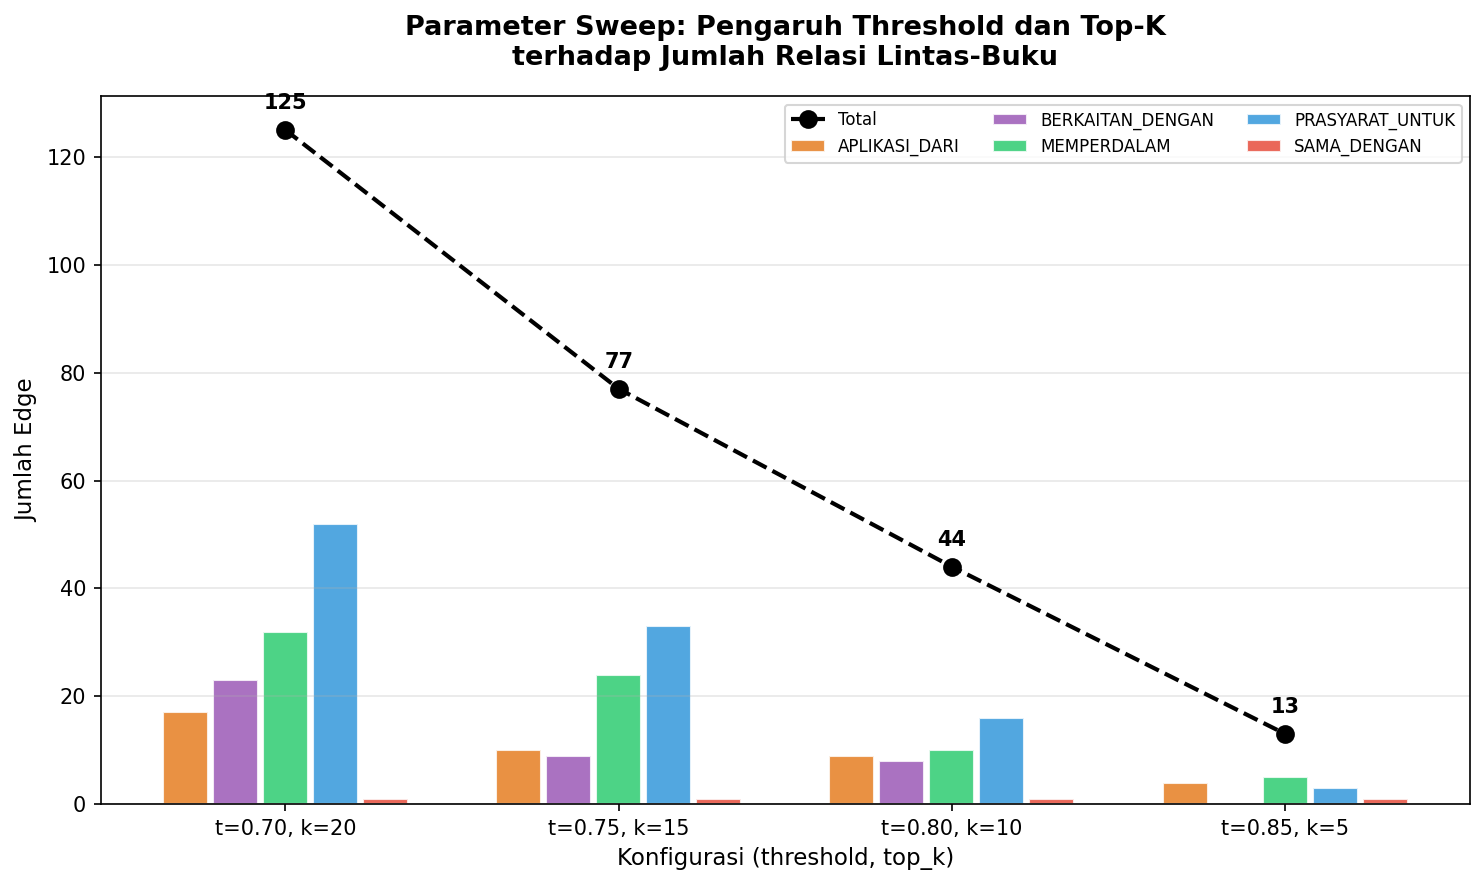
\includegraphics[width=\maxwidth]{images/media/image3.png}
  \caption{\textit{Parameter sweep}: pengaruh \textit{threshold} dan top-$k$ terhadap
    jumlah relasi lintas-buku yang ditemukan.}
  \label{fig:param-sweep}
\end{figure}

\begin{longtable}{@{}
  >{\raggedright\arraybackslash}p{0.40\linewidth}
  >{\raggedright\arraybackslash}p{0.54\linewidth}@{}}
\caption{Jumlah relasi lintas-buku per konfigurasi \textit{parameter sweep}.}
\label{tab:param-sweep}\\
\toprule
\textbf{Konfigurasi (threshold / top-$k$)} & \textbf{Jumlah relasi} \\
\midrule
\endhead
0{,}70 / $k$=20 (permisif --- konfigurasi final) & 125 \\
0{,}75 / $k$=15                                   & 72  \\
0{,}80 / $k$=10                                   & 42  \\
0{,}85 / $k$=5 (paling ketat)                     & 14  \\
\bottomrule
\end{longtable}

\begin{figure}[htbp]
  \centering
  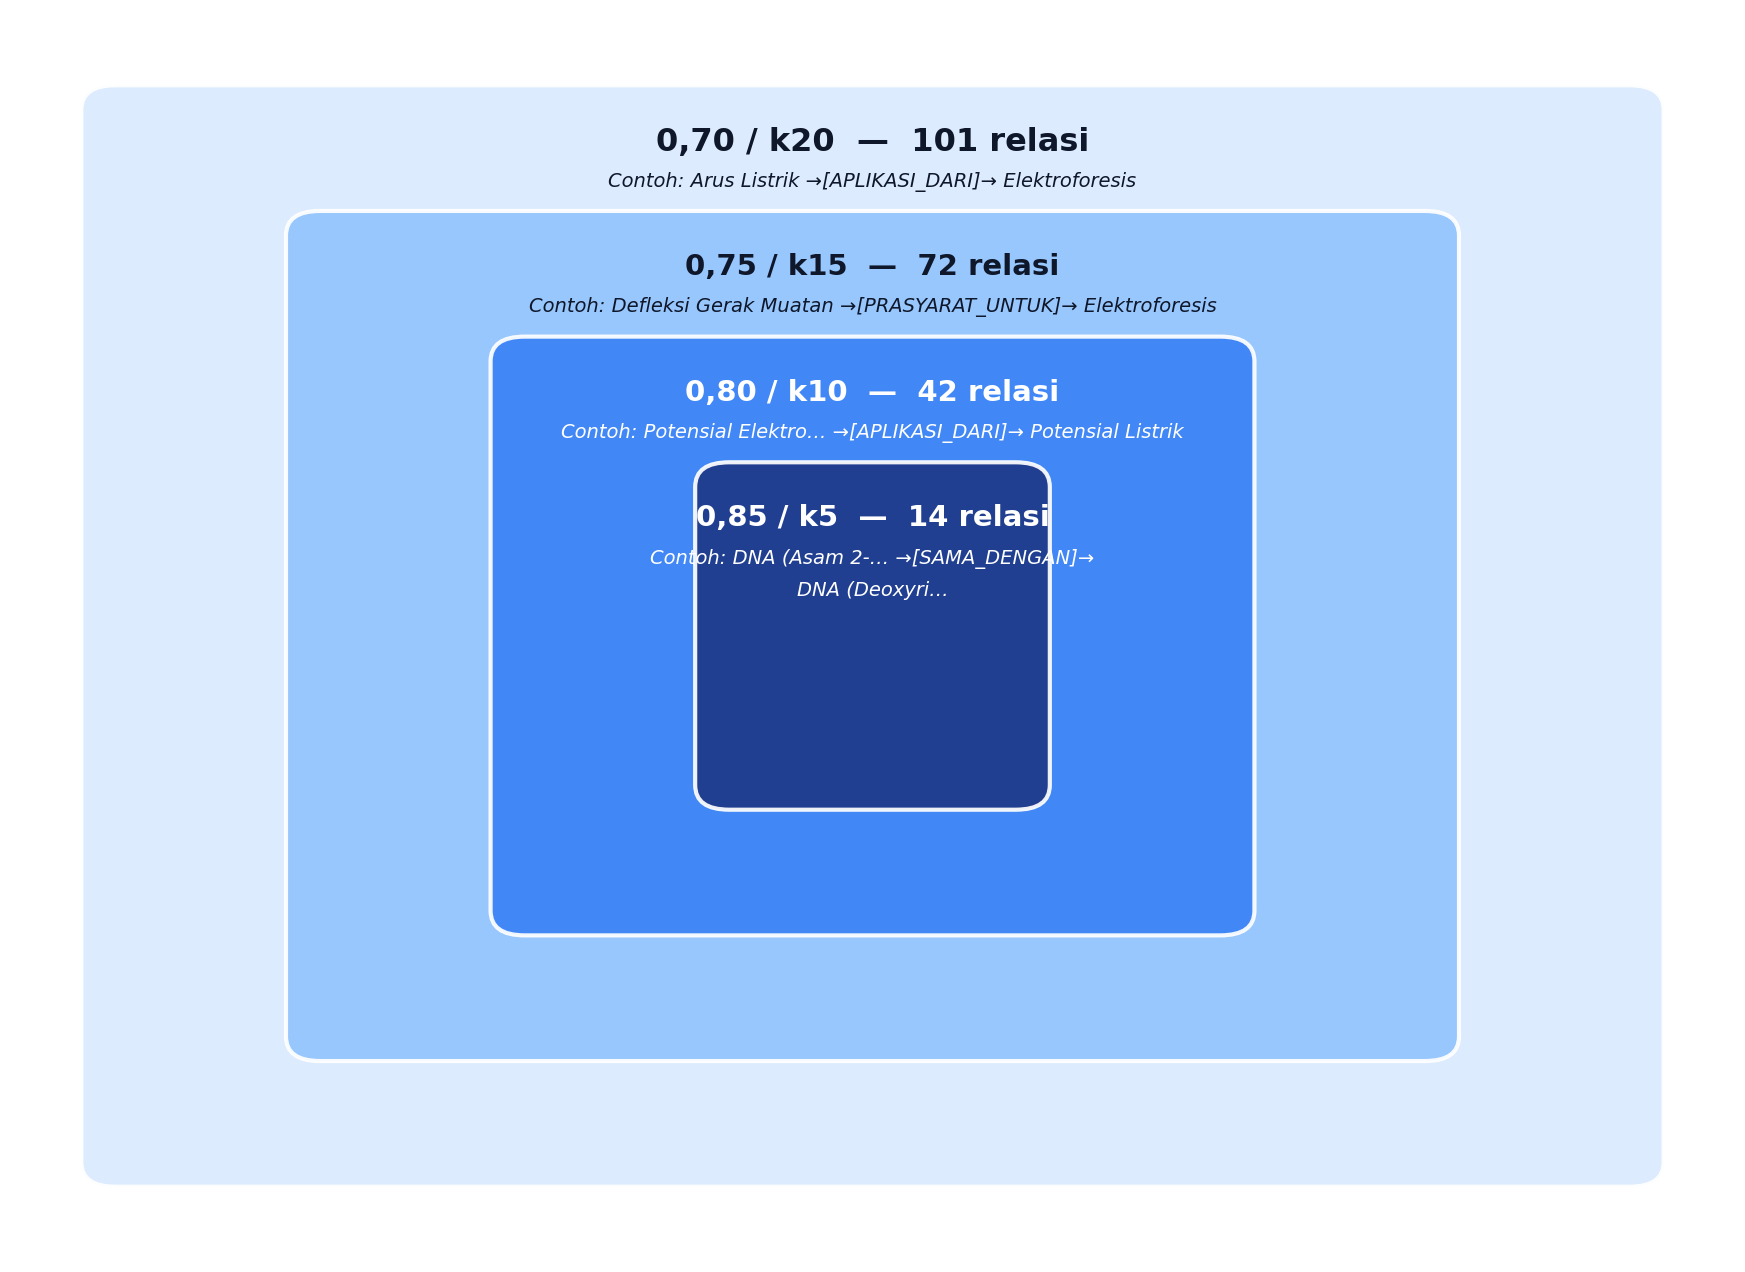
\includegraphics[width=\maxwidth]{images/media/image4.png}
  \caption{Struktur bersarang (\textit{nested}) hasil \textit{parameter sweep} relasi
    lintas-buku. Setiap konfigurasi yang lebih ketat merupakan himpunan bagian
    (\textit{subset}) dari konfigurasi yang lebih permisif.}
  \label{fig:nested-sweep}
\end{figure}

Konfigurasi membentuk himpunan bersarang: setiap konfigurasi yang lebih
ketat merupakan himpunan bagian dari yang lebih permisif. Pengetatan
parameter dengan demikian berfungsi sebagai kompromi \textit{recall} ---
menukar cakupan relasi (lebih banyak interkoneksi ditemukan) dengan
selektivitas (hanya pasangan berkemiripan tertinggi yang dipertahankan).
Sebagaimana akan dibahas pada Subbab~\ref{subsubsec:kualitas}, pengetatan ini menurunkan
kuantitas relasi tetapi \textbf{tidak} memperbaiki ketepatan arah relasi.

% ──────────────────────────────────────────
\subsubsection{Kualitas Relasi Lintas-Buku yang Ditemukan}\label{subsubsec:kualitas}
% ──────────────────────────────────────────

Pada konfigurasi final (threshold = 0{,}70; top-$k$ = 20; \textit{scope}
lintas-mapel), \textit{pipeline} menemukan 125 relasi lintas-buku. Distribusi
tipe relasi (Gambar~\ref{fig:relasi-distribusi}) didominasi PRASYARAT\_UNTUK (57 \textit{edge}, 45{,}6\%), diikuti
MEMPERDALAM (31 \textit{edge}, 24{,}8\%), BERKAITAN\_DENGAN (21 \textit{edge}, 16{,}8\%),
APLIKASI\_DARI (15 \textit{edge}, 12{,}0\%), dan SAMA\_DENGAN (1 \textit{edge}, 0{,}8\%).
Dominasi PRASYARAT\_UNTUK mengindikasikan bahwa jembatan lintas-disiplin
pada kurikulum sains kelas XII lebih banyak bersifat prasyarat pengetahuan
daripada aplikasi atau analogi. Dari 125 relasi, 8 \textit{edge} berkonfidens
$< 0{,}5$ (seluruhnya BERKAITAN\_DENGAN) dikeluarkan dari survei validasi
utama, menyisakan 117 relasi yang dinilai pakar.

\begin{figure}[htbp]
  \centering
  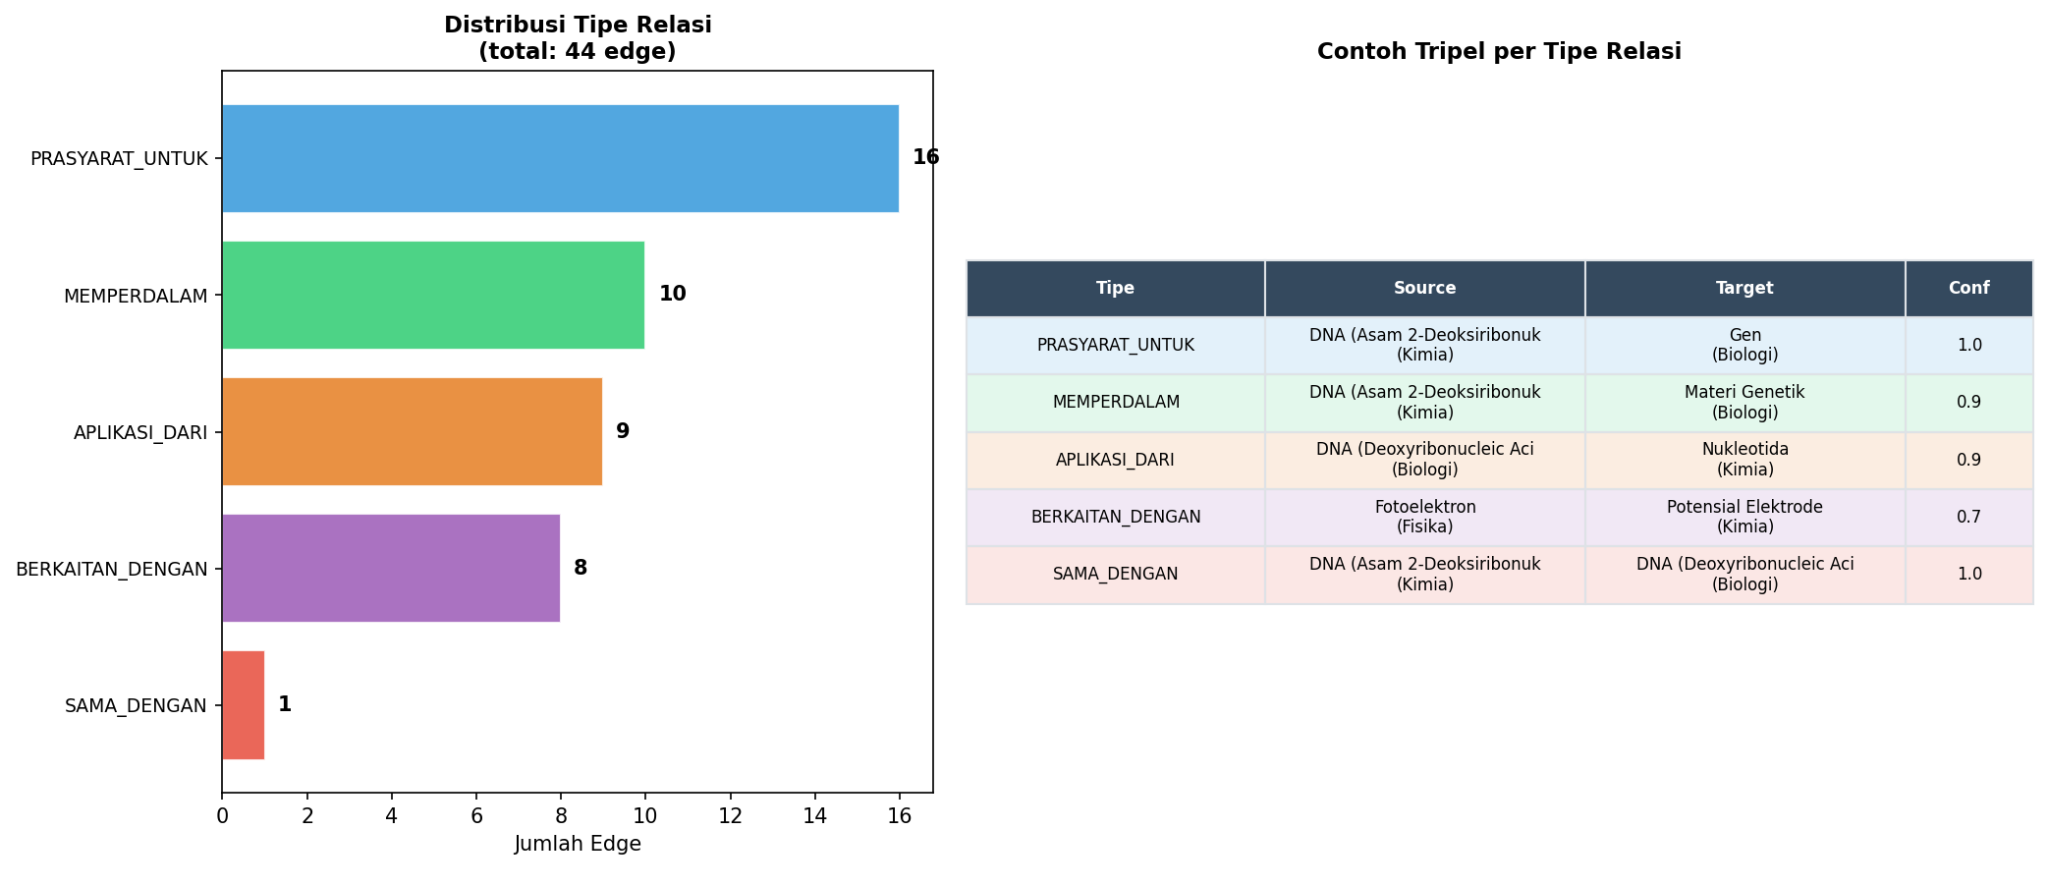
\includegraphics[width=\maxwidth]{images/media/image22.png}
  \caption{Distribusi tipe relasi lintas-buku hasil klasifikasi LLM beserta contoh triple per tipe.}
  \label{fig:relasi-distribusi}
\end{figure}

Dari 125 \textit{edge}, 20 (16\%) memiliki skor \textit{confidence} = 1{,}0, menunjukkan
keyakinan tinggi LLM terhadap relasi tersebut. Contoh relasi dengan
\textit{confidence} tertinggi meliputi:

\begin{itemize}
  \item DNA (Asam 2-Deoksiribonukleat) [Kimia] $\to$ Gen [Biologi]:
    PRASYARAT\_UNTUK (conf = 1{,}0). Pemahaman struktur kimia DNA merupakan
    fondasi untuk memahami fungsi gen secara biologis.
  \item Potensial Elektrode [Kimia] $\to$ Potensial Listrik [Fisika]:
    APLIKASI\_DARI (conf = 1{,}0). Konsep potensial elektrode dalam
    elektrokimia merupakan aplikasi langsung dari konsep potensial listrik
    dalam fisika.
  \item Enzim [Biologi] $\to$ Protein [Kimia]: APLIKASI\_DARI (conf = 1{,}0).
    Enzim merupakan manifestasi fungsional dari protein dalam konteks biologis.
  \item Fosforilasi Oksidatif [Biologi] $\to$ Oksidasi [Kimia]:
    PRASYARAT\_UNTUK (conf = 1{,}0). Pemahaman reaksi oksidasi secara kimia
    diperlukan sebelum mempelajari fosforilasi oksidatif dalam metabolisme.
\end{itemize}

Satu-satunya relasi bertipe SAMA\_DENGAN yang ditemukan adalah DNA (Asam
2-Deoksiribonukleat) [Kimia] $\leftrightarrow$ DNA (Deoxyribonucleic Acid)
[Biologi] dengan \textit{confidence} 1{,}0. Temuan ini mengonfirmasi bahwa
\textit{pipeline} mampu mendeteksi entitas identik yang diajarkan di dua disiplin
berbeda dengan terminologi yang sedikit berbeda.

\textbf{Validasi Pakar atas Relasi Lintas-Buku}

Untuk menilai kualitas relasi lintas-buku secara langsung, himpunan
relasi hasil \textit{Graph Completion} divalidasi oleh pakar melalui instrumen
survei lintas-buku (Fase 2). Setiap relasi A --[\textsc{tipe}]$\to$ B dinilai
pada tiga aspek terpisah: (1) \textit{validitas} --- apakah konsep A dan B
benar-benar berkaitan (Ya/Tidak); (2) \textit{ketepatan tipe} --- apakah
label relasi yang diusulkan tepat (Benar/Salah); dan (3) \textit{ketepatan
arah} --- apakah arah relasi A$\to$B sudah benar (Benar/Terbalik/NA untuk
relasi simetris). Penyajian bersifat \textit{score-blind} dan acak agar
pakar tidak ter-\textit{anchor} pada skor kepercayaan model.

Validasi dilakukan melalui diskusi panel atas seluruh 117 relasi kandidat
pada konfigurasi final ($\tau$=0{,}70, $k$=20). Hasil per-aspek menunjukkan
\textbf{validitas 99{,}1\%} (116/117), \textbf{ketepatan tipe 98{,}3\%}
(115/117; dua relasi salah tipe: LB008 dan LB074), namun \textbf{ketepatan
arah 75{,}9\%} (88/116; 28 terbalik, 1 NA untuk relasi simetris LB085).

Temuan utama validasi ini adalah bahwa \textbf{arah relasi merupakan
sumber kesalahan dominan}, bukan keberadaan atau tipe relasi. Sistem
sangat andal dalam \textit{menemukan} keterkaitan lintas-buku yang nyata
(99{,}1\%) dan dalam \textit{melabeli} tipenya (98{,}3\%), tetapi salah
menentukan arah pada hampir satu dari empat relasi. Kesalahan arah ini
bersifat sistematis: 26 dari 28 relasi terbalik berasal dari pasangan
Biologi\,$\leftrightarrow$\,Kimia: LLM cenderung menempatkan konsep
Biologi sebagai sumber, padahal arah yang benar umumnya
Kimia$\to$Biologi --- konsep kimia berperan sebagai prasyarat/fondasi
yang \textit{diperdalam} atau \textit{dibutuhkan} oleh proses biologis.
Tipe MEMPERDALAM paling rentan (ketepatan arah 60\%: 18 Benar, 12
Terbalik), disusul APLIKASI\_DARI (73\%) dan PRASYARAT\_UNTUK (79\%),
sementara tipe simetris BERKAITAN\_DENGAN dan SAMA\_DENGAN mencapai
100\% karena arah tidak relevan secara semantik.

Validitas relasi telah mendekati titik jenuh bahkan pada ambang permisif
0{,}70. Dengan demikian pengetatan parameter (lihat
Gambar~\ref{fig:param-sweep}) terutama menukar \textit{recall} (jumlah
relasi yang ditemukan) dengan \textit{noise}, bukan meningkatkan presisi
keberadaan relasi. Konfigurasi 0{,}75 dan 0{,}80 belum divalidasi pakar,
sehingga klaim tentang kualitas di seluruh rentang parameter belum dapat
ditegaskan. Kesalahan arah bukan persoalan ambang --- relasi terbalik
tetap merupakan pasangan berkemiripan tinggi yang valid secara semantik
--- sehingga penanganannya memerlukan perbaikan pada \textit{prompt}
klasifikasi atau kanonikalisasi arah pasca-proses, bukan penyetelan
\textit{threshold}.

\begin{longtable}{@{}
  >{\raggedright\arraybackslash}p{0.20\linewidth}
  >{\raggedright\arraybackslash}p{0.16\linewidth}
  >{\raggedright\arraybackslash}p{0.16\linewidth}
  >{\raggedright\arraybackslash}p{0.20\linewidth}
  >{\raggedright\arraybackslash}p{0.20\linewidth}@{}}
\caption{Hasil validasi pakar atas relasi lintas-buku per konfigurasi parameter.}
\label{tab:validasi-sweep}\\
\toprule
\textbf{Konfigurasi} & \textbf{Jumlah edge} & \textbf{Validitas} & \textbf{Ketepatan tipe} & \textbf{Ketepatan arah} \\
\midrule
\endhead
0{,}70 / $k$=20 (disurvei, $n$=117) & 125 & 99{,}1\% & 98{,}3\% & 75{,}9\% \\
0{,}75 / $k$=15 (belum divalidasi) & 72  & ---  & ---  & ---  \\
0{,}80 / $k$=10 (belum divalidasi) & 42  & ---  & ---  & ---  \\
\bottomrule
\end{longtable}

% ──────────────────────────────────────────
\subsubsection{Analisis Relasi Berpotensi False Positive}\label{subsubsec:false-positive}
% ──────────────────────────────────────────

Sebanyak 9 \textit{edge} memiliki \textit{confidence} $< 0{,}7$ (8 di antaranya $< 0{,}5$),
yang mengindikasikan potensi \textit{false positive}:

\begin{itemize}
  \item Gerbang Logika Dasar [Fisika] $\leftrightarrow$ Notasi Sel Standar [Kimia]:
    BERKAITAN\_DENGAN (conf = 0{,}2). Relasi ini merupakan contoh \textit{false
    positive} --- kemiripan \textit{embedding} terjadi akibat kedua konsep sama-sama
    melibatkan notasi simbolik, namun tidak ada hubungan kurikuler bermakna.
  \item Klasifikasi Semikonduktor [Fisika] $\leftrightarrow$ Polimer Anorganik [Kimia]:
    BERKAITAN\_DENGAN (conf = 0{,}4). Kemiripan kemungkinan didorong oleh kesamaan
    konteks material/bahan, namun hubungan substantifnya lemah.
  \item Efek Fotolistrik [Fisika] $\leftrightarrow$ Fotosintesis [Biologi]:
    BERKAITAN\_DENGAN (conf = 0{,}7). Keduanya melibatkan interaksi foton dengan
    materi, tetapi mekanisme dan konteksnya sangat berbeda.
\end{itemize}

Temuan ini mengonfirmasi peran penting label \textit{fallback} BERKAITAN\_DENGAN
sebagai penanda relasi yang lemah atau ambigu. Dari 21 \textit{edge} bertipe
BERKAITAN\_DENGAN, mayoritas memiliki \textit{confidence} lebih rendah dibandingkan
tipe lainnya, menunjukkan bahwa LLM menggunakan label ini ketika tidak yakin
terhadap arah atau tipe relasi yang lebih spesifik.

% ──────────────────────────────────────────
\subsubsection{Analisis Pola Kesalahan Ekstraksi (Error Analysis)}\label{subsubsec:error-analysis}
% ──────────────────────────────────────────

Analisis \textit{feedback} pakar mengungkapkan beberapa pola kesalahan sistematis
pada \textit{pipeline} ekstraksi LLM:

\textbf{Kesalahan faktual agen biologis.} Pada Kimia, \textit{triple} mengenai produksi
etanol menyatakan ``bakteri memfermentasi karbohidrat'' padahal seharusnya
``ragi (\textit{Saccharomyces cerevisiae})''. Kesalahan ini termasuk dalam kategori
\textit{hallucination} faktual sebagaimana diidentifikasi pada Subbab~\ref{subsec:kg-ontologi}.

\textbf{Pencampuran konsep teknis.} \textit{Triple} mengenai pemurnian tembaga menyatakan
bahwa \textit{electroplating} digunakan untuk pemurnian tembaga, padahal proses yang
benar adalah \textit{elektrorefining}. Kedua konsep memang melibatkan elektrolisis,
namun tujuan dan mekanismenya berbeda.

\textbf{Definisi yang terlalu luas.} Expert-fisika-6 mencatat sejumlah definisi yang
menimbulkan bias, misalnya definisi konstanta Coulomb yang ``terlalu luas'' tanpa
menyebutkan jenis konstantanya. Umpan balik umum dari penilai ini menekankan:
``Penjelasannya dipastikan jangan ada bias\ldots Lebih ke penulisan, notasi, dan
definisi nya perlu dicek dan dirapihkan kembali.''

\textbf{Under-extraction formula dan rumus.} Expert-fisika-4 mengusulkan 15
\textit{missing triples}; 10 di antaranya (67\%) merupakan formula/rumus
yang tidak berhasil diekstrak oleh LLM. Ini menunjukkan bahwa LLM cenderung
mengekstrak konsep deskriptif namun melewatkan relasi kuantitatif berbasis
persamaan matematika. Contoh: rumus efisiensi transformator ($\eta$), nilai
efektif arus AC ($I_\text{ef}$), panjang gelombang minimum sinar-X
($\lambda_\text{min}$), dan rumus peluruhan radioaktif ($N_t$).

% ──────────────────────────────────────────
\subsubsection{Analisis Koreksi dan Kategori Feedback}\label{subsubsec:feedback}
% ──────────────────────────────────────────

Dari 222 komentar yang diberikan Expert-fisika-4, analisis tematik
menunjukkan distribusi:

\begin{itemize}
  \item Penjelasan/konfirmasi rumus: 78 komentar (35\%) --- mayoritas bersifat
    validasi bahwa rumus sudah benar.
  \item Klarifikasi definisi: 52 komentar (23\%) --- penajaman definisi konsep.
  \item Koreksi notasi: 45 komentar (20\%) --- perbaikan penulisan simbol dan satuan.
  \item Peringatan bias: 28 komentar (13\%) --- potensi \textit{misleading} pada pembaca.
  \item Penambahan konteks: 19 komentar (9\%) --- konteks tambahan yang perlu disertakan.
\end{itemize}

Pola ini mengindikasikan bahwa kekuatan utama LLM terletak pada
ekstraksi struktur konseptual (87\% komentar bernilai konfirmasi atau
netral), namun kelemahan terletak pada presisi notasi dan formulasi
matematis. Perlu dicatat bahwa angka 87\% dihitung dari proporsi komentar
konfirmasi/klarifikasi terhadap total 222 komentar Expert-fisika-4, bukan
dari jumlah triple yang dinilai; denominator kedua ukuran tersebut berbeda.

% ──────────────────────────────────────────
\subsubsection{Dampak KGC terhadap Kualitas Graf}\label{subsubsec:dampak-kgc}
% ──────────────────────────────────────────

\textit{Pipeline} KGC berhasil menambahkan 125 jembatan lintas-buku antar-mata
pelajaran yang sebelumnya tidak ada. Secara kualitatif, mayoritas relasi
ini bermakna pedagogis dan dapat dipertanggungjawabkan secara ilmiah.
Namun, keberadaan \textit{false positive} (terutama pada \textit{confidence} rendah)
menggarisbawahi pentingnya \textit{threshold} yang tepat dan validasi pakar
sebagai filter akhir.

% ────────────────────────────────────────────────────────────
\subsection{Analisis Komparatif Antar-Domain Sains}\label{subsec:komparatif}
% ────────────────────────────────────────────────────────────

Bagian ini membandingkan ketiga domain sains dari dua sisi: \textbf{pola
interkoneksi} antar-mata pelajaran (berapa banyak jembatan lintas-buku
yang terbentuk antar pasangan disiplin) dan \textbf{kualitas ekstraksi}
per domain.

\begin{figure}[htbp]
  \centering
  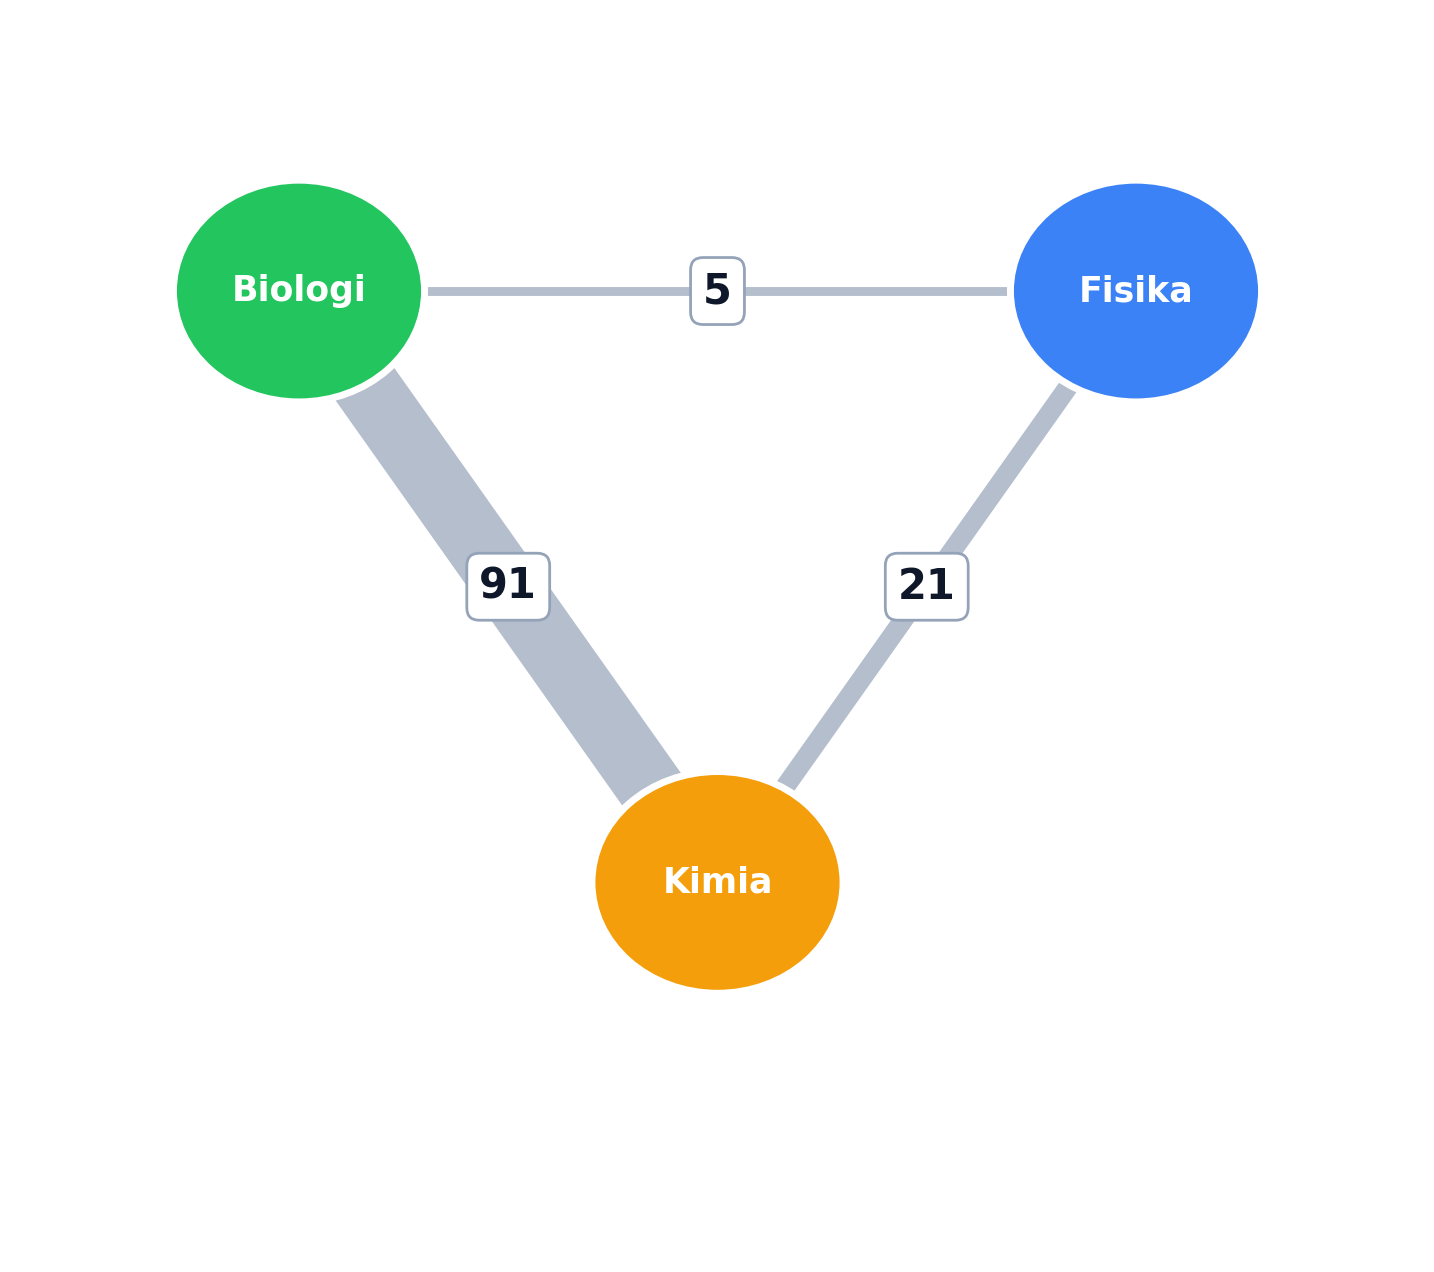
\includegraphics[width=0.85\linewidth]{images/media/image14.png}
  \caption{\textit{Inter-domain bridge graph}. Setiap simpul adalah satu mata pelajaran;
    ketebalan dan label sisi menyatakan jumlah relasi lintas-buku yang ditemukan
    antar pasangan disiplin (dari 117 relasi yang disurvei pada konfigurasi final).}
  \label{fig:bridge-graph}
\end{figure}

Distribusi jembatan lintas-disiplin sangat tidak merata. Pasangan
Biologi--Kimia mendominasi (91 relasi, 78\%), diikuti Fisika--Kimia (21
relasi, 18\%), sedangkan Biologi--Fisika nyaris tidak terhubung (5
relasi, 4\%). Pola ini menempatkan Kimia sebagai poros (\textit{hub}) yang
menjembatani kedua disiplin lain. Temuan ini konsisten secara pedagogis:
tumpang-tindih molekuler dan biokimiawi (DNA, protein, enzim, reaksi
redoks) membuat Biologi dan Kimia berbagi banyak konsep dasar, sementara
keterkaitan Fisika sebagian besar terbatas pada elektrokimia (arus dan
potensial listrik $\leftrightarrow$ sel elektrokimia). Sifat Fisika yang lebih
abstrak-matematis menjadikannya domain paling terisolasi dalam jaringan
konsep kurikulum kelas XII.

Dari sisi kualitas ekstraksi (validasi Fase 1), terdapat perbedaan
antar-domain:

\begin{longtable}{@{}
  >{\raggedright\arraybackslash}p{0.15\linewidth}
  >{\raggedright\arraybackslash}p{0.50\linewidth}
  >{\raggedright\arraybackslash}p{0.30\linewidth}@{}}
\caption{Presisi ekstraksi per domain sains (Fase 1 validasi pakar).}
\label{tab:komparatif-domain}\\
\toprule
\textbf{Domain} & \textbf{Presisi ekstraksi (Fase 1)} & \textbf{Catatan} \\
\midrule
\endhead
Biologi & $\sim$0{,}95--0{,}97 & paling konsisten; konsep deskriptif-naratif \\
Fisika  & $\sim$0{,}86--0{,}99 & rentang lebar; lemah pada relasi kuantitatif/rumus \\
Kimia   & $\sim$0{,}82--0{,}92 & kesalahan terbanyak pada terminologi proses \\
\bottomrule
\end{longtable}

Perbedaan ini selaras dengan analisis kesalahan pada Subbab~\ref{subsubsec:error-analysis}:
kelemahan utama pada Fisika adalah \textbf{under-extraction rumus} (67\%
\textit{missing triples} Fisika berupa formula), sedangkan Kimia rentan pada
\textbf{pencampuran konsep teknis}. Biologi---yang materinya lebih
bersifat deskriptif---paling sesuai dengan kekuatan LLM dalam mengekstrak
struktur konseptual.

\ifSubfilesClassLoaded{\printbibliography[title={Daftar Pustaka}]}{}

\end{document}
